\chapter{क्वांटम भौतिकी का परिचय}\label{ch:b1:quantum-introduction}

किसी साफ़ धातु पर पराबैंगनी प्रकाश डालिए और इलेक्ट्रॉन तुरंत उड़ निकलते हैं,
ऐसी ऊर्जा के साथ जो प्रकाश के रंग पर निर्भर करती है और उसकी चमक पर बिलकुल
नहीं; और लाल प्रकाश डालिए तो कुछ भी बाहर नहीं आता, बत्ती चाहे कितनी भी तेज़
हो। इलेक्ट्रॉनों को एक-एक करके दो झिर्रियों से भेजिए और वे बिंदुओं की तरह
आ गिरते हैं, हर एक किसी एक ही जगह --- और हज़ारों के बाद वे बिंदु मिलकर किसी
तरंग की फ्रिंजें बना देते हैं। इनमें से कोई भी तथ्य पहले उनतीस अध्यायों की
भौतिकी में नहीं बैठता। यह आख़िरी अध्याय वे विचार लाता है जो इनमें बैठते
हैं: प्रकाश क्वांटमों में आता है, यानी फ़ोटॉनों में; द्रव्य की एक
तरंगदैर्घ्य होती है; जो संचरित होता है वह कोई \omterm{def:b1:wave-propagation:signal}{आयाम} है जिसका वर्ग एक
प्रायिकता है; स्थिति और संवेग दोनों एक साथ तीखे नहीं हो सकते; और कोई बंद
कण केवल कुछ ही ऊर्जाएँ रख सकता है --- इसीलिए परमाणुओं के आकार होते हैं,
वर्णक्रमों में रेखाएँ होती हैं, और कुछ नैनोमीटर का अर्धचालक का कोई कण अपने
व्यास से तय हुए रंग में चमकता है।

\section{फ़ोटॉन}

\begin{theorem}[प्लांक--आइंस्टाइन संबंध]\label{thm:b1:quantum-introduction:photon}
\index{फ़ोटॉन}\index{प्लांक नियतांक}
आवृत्ति $\nu$ और तरंगदैर्घ्य $\lambda$ का प्रकाश पदार्थ के साथ ऊर्जा का
आदान-प्रदान केवल क्वांटमों में करता है, यानी \emph{फ़ोटॉनों} में, जिनकी
ऊर्जा और संवेग ये हैं
\[
E = h\nu = \frac{hc}{\lambda} , \qquad p = \frac{h}{\lambda} = \frac{E}{c} ,
\]
जहाँ \emph{\omterm{thm:b1:quantum-introduction:photon}{प्लांक नियतांक}} $h = \qty{6.626e-34}{J.s}$ है ($\hbar = h/2\pi =
\qty{1.055e-34}{J.s}$)। काम का: $hc = \qty{1240}{eV.nm}$ --- यानी
\qty{620}{nm} का कोई फ़ोटॉन \qty{2}{eV} ले जाता है।
\end{theorem}
\admitted

\begin{proposition}[प्रकाश-विद्युत प्रभाव]\label{prop:b1:quantum-introduction:photoelectric}
\index{प्रकाश-विद्युत प्रभाव}\index{कार्य-फलन}\index{निरोधी विभव}
\emph{कार्य-फलन} $W$ की किसी धातु पर पड़ता प्रकाश (यह वह ऊर्जा है जो उसके
सबसे ढीले बँधे इलेक्ट्रॉनों को बाँधे रखती है, कुछ \omterm{def:b1:charged-particles:eV}{इलेक्ट्रॉन-वोल्ट}) ऐसे
इलेक्ट्रॉन निकालता है जिनकी अधिकतम \omterm{thm:b1:work-and-energy:ke}{गतिज ऊर्जा} यह है
\[
E_{k,\max} = h\nu - W ,
\]
अतः केवल \emph{देहली} $\nu_0 = W/h$ के ऊपर ही, और तत्काल, ऐसी ऊर्जा के साथ
जो तीव्रता से स्वतंत्र है; तीव्रता तो प्रति सेकंड इलेक्ट्रॉनों की
\emph{संख्या} तय करती है। जो \emph{\omterm{prop:b1:quantum-introduction:photoelectric}{निरोधी विभव}}
$V_s$ धारा को ठीक-ठीक रोक देता है वह $E_{k,\max} = eV_s$ माप देता है, और
$V_s$ का आलेख, $\nu$ के सामने, $h/e$ ढाल की सीधी रेखा है --- इसी तरह मिलिकन
ने $h$ मापा था।
\end{proposition}

\begin{proof}
हर फ़ोटॉन किसी एक इलेक्ट्रॉन से सोख लिया जाता है, जो अधिक से अधिक
$h\nu - W$ रख पाता है; कोई तरंग तो ऊर्जा हर इलेक्ट्रॉन को लगातार देती
रहती, ऊर्जा तीव्रता के साथ बढ़ती, और कोई कमज़ोर प्रकाश किसी एक परमाणु पर
$W$ जमा करने में घंटों लेता (\cref{pb:b1:quantum-introduction:1}) ---
और इनमें से कुछ भी देखा नहीं जाता। आइंस्टाइन की व्याख्या (1905) यहाँ नियम
के रूप में स्वीकृत है।
\end{proof}

\begin{omfigure}
\begin{tikzpicture}[font=\small, x=1cm, y=1cm, >=Stealth]
  % apparatus
  \draw[fill=omExo!25, draw=omExo, thick] (-2.2,-1.2) rectangle (-1.7,1.2); \node[font=\footnotesize] at (-1.95,-1.5) {कैथोड};
  \draw[omThm, thick] (1.7,-1.2) -- (1.7,1.2); \node[font=\footnotesize] at (1.7,-1.5) {ऐनोड};
  \foreach \y in {0.6,0.2,-0.2} \draw[omProp, ->, decorate, decoration={snake, amplitude=1.5pt, segment length=4pt, post length=3pt}] (-3.8,\y+0.6) -- (-2.25,\y);
  \node[omProp, font=\footnotesize] at (-3.6,1.55) {प्रकाश, $\nu$};
  \foreach \y in {0.7,0,-0.7} \draw[omDef, ->] (-1.65,\y) -- (0.4,\y);
  \node[omDef, font=\footnotesize] at (0,1.0) {$E_k \leq h\nu - W$};
  \draw (-1.95,-1.2) -- (-1.95,-2.2) -- (1.7,-2.2) -- (1.7,-1.2);
  \draw[fill=white] (-0.6,-2.45) rectangle (0.4,-1.95); \node[font=\footnotesize] at (-0.1,-2.2) {$V_s$};
  \node[font=\footnotesize] at (-0.1,-2.75) {ऐनोड $-V_s$ पर रखा गया: धारा ठीक शून्य};
\end{tikzpicture}\hfill
\begin{tikzpicture}
\begin{axis}[omaxis, axis x line=bottom, axis y line=left, width=7.4cm, height=5.4cm,
    xlabel={$\nu$ ($10^{14}$ Hz)}, ylabel={$V_s$ (V)},
    xlabel style={at={(axis description cs:1.0,0.0)}, anchor=north east, yshift=-10pt},
    xmin=0, xmax=12.5, ymin=0, ymax=3, xtick={2,4,...,12}, ytick={1,2,3}, samples=2, clip=false]
  \addplot[omDef, thick, domain=5.32:12] {0.4136*x-2.2};
  \addplot[only marks, mark=*, mark size=1.6pt, omThm] coordinates {(6,0.30) (7,0.69) (8,1.13) (9,1.50) (11,2.36)};
  \addplot[omDef, dashed, thin, domain=3.6:5.32] {0.4136*x-2.2};
  \node[font=\footnotesize, omDef, anchor=east] at (axis cs:3.4,-0.6) {अंतःखंड $-W/e$};
  \node[font=\footnotesize, anchor=south] at (axis cs:5.32,0.05) {$\nu_0$};
  \node[font=\footnotesize, omDef, anchor=west] at (axis cs:8.4,0.9) {ढाल $h/e$};
\end{axis}
\end{tikzpicture}

{\small बाएँ: प्रकाश-विद्युत सेल --- प्रकाश कैथोड से इलेक्ट्रॉन मुक्त करता
है; और उन्हें रोक देने भर की उलटी वोल्टता $V_s$ उनकी अधिकतम ऊर्जा माप देती
है। दाएँ: आवृत्ति के सामने \omterm{prop:b1:quantum-introduction:photoelectric}{निरोधी विभव} हर धातु के लिए $h/e$ ढाल की सीधी
रेखा है; अंतःखंड कार्य-फलन देता है और देहली न्यूनतम आवृत्ति।}
\end{omfigure}

\begin{example}[परिमाण की कोटियाँ]\label{ex:b1:quantum-introduction:orders}
कोई दृश्य फ़ोटॉन: \qty{2}{eV}; \qty{0.1}{nm} का कोई X-किरण फ़ोटॉन: \qty{12}{keV};
\qty{100}{MHz} पर कोई रेडियो फ़ोटॉन: \qty{4e-7}{eV}। \qty{1}{mW} का कोई लाल
लेज़र प्रति सेकंड $10^{-3}/(3.1 \times 10^{-19}) = 3 \times 10^{15}$ फ़ोटॉन
छोड़ता है; और \qty{100}{MHz} पर \qty{1}{pW} उठाता कोई रेडियो एंटीना प्रति
सेकंड $10^{13}$ पाता है --- इतने सारे, इतने छोटे, कि हर प्रयोजन के लिए तरंग
वाला वर्णन ही यथार्थ बैठता है; जबकि आँख सौ भर फ़ोटॉनों की कौंध दर्ज कर लेती
है। प्रकाश की क्वांटम प्रकृति तभी दिखती है जब फ़ोटॉन थोड़े हों या ऊर्जावान:
प्रकाश-विद्युत सेल, X-किरण संसूचक, किसी धुँधले छायाचित्र के दाने।
\end{example}

\begin{remark}[कॉम्पटन प्रकीर्णन]\label{rem:b1:quantum-introduction:compton}
\index{कॉम्पटन प्रकीर्णन}
किसी मुक्त इलेक्ट्रॉन से टकराकर लौटता कोई फ़ोटॉन संवेग वैसे ही हस्तांतरित
करता है जैसे कोई बिलियर्ड गेंद: उसकी तरंगदैर्घ्य $\Delta\lambda = \frac{h}{m_ec}(1 -
\cos\theta)$ से बढ़ जाती है, जहाँ $h/m_ec = \qty{2.43}{pm}$ (स्वीकृत --- यह
कोई आपेक्षिक संघट्ट है, वर्ष 2)। प्रकाश के लिए यह अदृश्य है ($\Delta\lambda/\lambda \sim 10^{-5}$),
पर X-किरणों के लिए $20\%$ का प्रभाव है, और यही वह प्रयोग था जिसने (1923 में)
संदेह करने वालों को मना लिया कि फ़ोटॉन संवेग $h/\lambda$ ले जाता है।
\end{remark}

\section{द्रव्य तरंगें}

\begin{theorem}[दे ब्रॉय]\label{thm:b1:quantum-introduction:debroglie}
\index{दे ब्रॉय तरंगदैर्घ्य}\index{द्रव्य तरंग}
संवेग $p$ का कोई कण इस तरंगदैर्घ्य की तरंग की तरह संचरित होता है
\[
\lambda = \frac{h}{p} ,
\]
और उसी के अनुसार विवर्तन तथा व्यतिकरण दिखाता है: किसी रवे पर इलेक्ट्रॉन
(डेविसन और जर्मर, 1927), दो झिर्रियों से होकर (योंसन, 1961), न्यूट्रॉन,
परमाणु, और साठ कार्बन परमाणुओं के अणु। $U$ से त्वरित किसी इलेक्ट्रॉन के लिए,
$\lambda = h/\sqrt{2m_eeU} = \qty{1.23}{nm}/\sqrt{U/\unit{V}}$।
\end{theorem}
\admitted

\begin{example}[यह हमें कभी दिखा क्यों नहीं]\label{ex:b1:quantum-introduction:wavelengths}
\qty{100}{eV} का कोई इलेक्ट्रॉन: $\lambda = \qty{0.12}{nm}$, यानी किसी रवे
में परमाणुओं की दूरी --- इसीलिए विवर्तन, और इसीलिए इलेक्ट्रॉन \omterm{def:b1:optical-instruments:microscope}{सूक्ष्मदर्शी}।
कोई तापीय न्यूट्रॉन (\qty{0.025}{eV}): \qty{0.18}{nm}। और \qty{1}{m/s} पर
\qty{1}{g} की कोई गेंद: $\lambda = \qty{7e-31}{m}$, यानी किसी नाभिक से भी
$10^{20}$ गुना छोटी: कोई झिर्री, कोई रवा उसे कभी विवर्तित नहीं कर सकता।
द्रव्य की तरंग-प्रकृति सार्वभौम है; उसकी तरंगदैर्घ्य ही वह चीज़ है जो उसे
केवल हलके और धीमे के लिए दिखने देती है।
\end{example}

\begin{proposition}[अकेले कण ही फ्रिंजें बनाते हैं]\label{prop:b1:quantum-introduction:buildup}
\index{तरंग--कण द्वैत}
दो झिर्रियों से एक बार में एक भेजे गए इलेक्ट्रॉन (तोनोमुरा, 1989) हर एक
पर्दे पर एक ही बिंदु बनाते हैं, ऐसी जगह जिसका पूर्वानुमान नहीं किया जा
सकता; और वे बिंदु जमा होकर $h/p$ तरंगदैर्घ्य की किसी तरंग की दो-झिर्री
व्यतिकरण-आकृति बना देते हैं। एक झिर्री बंद कर दीजिए और फ्रिंजें मिट जाती
हैं --- वह आकृति इलेक्ट्रॉनों के आपस में व्यतिकरण से नहीं बनती, बल्कि हर
इलेक्ट्रॉन की अपनी तरंग के दोनों झिर्रियों से गुज़रने से। और यह पता कर
लेना कि कोई कण किस झिर्री से गया, भी फ्रिंजें मिटा देता है।
\end{proposition}
\admitted

\begin{omfigure}
\begin{tikzpicture}[font=\small, x=1cm, y=1cm]
  \begin{scope}
    \draw (-3.2,0) rectangle (3.2,1.3);
    \foreach \x/\y in {-0.42/0.13, -0.48/1.04, 1.15/0.56, 0.55/0.59, 0.60/0.75, -0.69/0.53, -0.22/0.63, 0.11/0.48, 0.98/1.01, 0.53/1.14, 0.15/0.07, 0.79/0.66, 0.45/0.89, -1.25/0.96, 0.00/0.26, -3.08/0.35, -0.16/1.17, 1.20/1.23, -0.61/0.47, -1.22/0.48, -1.91/0.66, 0.03/1.05, 1.17/0.88, -0.07/0.05, 0.75/0.82, -1.25/0.73, 1.23/0.86, 0.11/0.61, 3.06/1.17, -1.18/1.06, -0.46/0.38, 0.07/0.28, 0.15/0.50, 0.53/0.52, 0.65/0.06, 1.12/0.55, 1.07/1.16, 1.06/1.19, -1.17/0.38, -0.73/0.35, -0.04/1.16, -1.62/0.13, -0.53/0.79, 0.05/0.33, 0.53/1.17, 0.62/0.79, 1.14/0.27, -1.20/0.73, -0.49/1.03, 0.11/0.51, 0.64/0.71, -0.48/0.84, -0.07/0.33, -0.17/0.18, 0.07/0.10, 0.07/0.12, -0.78/1.19, -0.05/1.20, 0.04/0.43, 1.15/1.12} \fill[omDef] (\x,\y) circle (1.1pt);
    \node[font=\footnotesize] at (0,-0.35) {$60$ इलेक्ट्रॉन};
  \end{scope}
  \begin{scope}[yshift=-2.4cm]
    \draw (-3.2,0) rectangle (3.2,1.3);
    \foreach \x/\y in {-0.42/0.13, -0.48/1.04, 1.15/0.56, 0.55/0.59, 0.60/0.75, -0.69/0.53, -0.22/0.63, 0.11/0.48, 0.98/1.01, 0.53/1.14, 0.15/0.07, 0.79/0.66, 0.45/0.89, -1.25/0.96, 0.00/0.26, -3.08/0.35, -0.16/1.17, 1.20/1.23, -0.61/0.47, -1.22/0.48, -1.91/0.66, 0.03/1.05, 1.17/0.88, -0.07/0.05, 0.75/0.82, -1.25/0.73, 1.23/0.86, 0.11/0.61, 3.06/1.17, -1.18/1.06, -0.46/0.38, 0.07/0.28, 0.15/0.50, 0.53/0.52, 0.65/0.06, 1.12/0.55, 1.07/1.16, 1.06/1.19, -1.17/0.38, -0.73/0.35, -0.04/1.16, -1.62/0.13, -0.53/0.79, 0.05/0.33, 0.53/1.17, 0.62/0.79, 1.14/0.27, -1.20/0.73, -0.49/1.03, 0.11/0.51, 0.64/0.71, -0.48/0.84, -0.07/0.33, -0.17/0.18, 0.07/0.10, 0.07/0.12, -0.78/1.19, -0.05/1.20, 0.04/0.43, 1.15/1.120} \fill[omDef] (\x,\y) circle (1.1pt);
    \node[font=\footnotesize] at (0,-0.35) {$600$ इलेक्ट्रॉन};
  \end{scope}
  \begin{scope}[yshift=-4.6cm]
    \draw (-3.2,0) rectangle (3.2,1.3);
    \foreach \x/\y in {-0.02/0.94, 1.23/0.49, -1.77/0.11, 0.08/1.17, 0.58/0.98, -0.45/0.37, -1.29/0.96, -0.08/0.50, 0.27/1.07, -0.57/0.51, -0.57/0.28, -0.12/0.06, -0.00/0.62, 0.20/0.90, -0.01/0.81, -0.08/1.16, 0.57/0.90, -1.18/0.87, 0.47/0.79, 0.15/0.87, -0.77/1.01, -0.58/0.94, 0.06/1.13, 0.67/0.72, 1.29/0.61, 0.75/0.17, 1.23/0.09, -0.76/1.08, -1.29/0.68, -0.14/0.59, -1.13/0.63, 0.56/0.63, 0.13/0.95, 0.61/0.32, 0.05/0.24, -1.19/1.21, -0.68/0.95, 0.08/0.95, -1.25/0.14, -0.00/0.97, 0.46/1.23, -0.01/0.65, -0.49/0.26, 1.21/0.40, 0.62/1.16, -1.13/0.75, -0.47/0.32, 1.05/0.84, 0.73/0.44, 1.35/0.14, -0.07/0.11, -0.63/0.53, 0.02/0.24, 0.53/0.36, 0.35/0.73, 0.02/0.28, 0.63/1.12, 0.50/0.61, -0.21/0.94, -0.06/0.11, -0.09/1.09, 1.15/1.24, 1.06/0.65, 0.62/1.07, 0.74/0.41, -0.09/0.10, 0.75/0.06, -1.06/0.43, -0.55/0.75, 0.68/1.23, 0.06/1.07, 1.37/0.27, 0.48/0.42, -0.45/0.66, 1.22/0.12, 0.55/0.08, 1.17/0.85, 0.11/1.22, -0.13/0.86, 0.15/0.26, -0.55/0.94, 0.10/0.53, 1.26/0.83, -0.79/0.40, -0.04/0.23, 1.21/0.36, -0.14/0.08, -1.27/0.75, -1.29/0.23, 3.02/0.76, 0.62/1.20, 1.26/0.22, -1.16/0.83, -1.03/0.62, -0.02/1.12, -2.97/0.76, 0.12/0.98, -0.40/0.70, -0.57/0.09, -0.03/0.54, 1.74/0.33, 0.60/0.33, -0.61/0.36, -1.08/1.24, -0.58/0.49, 0.52/0.54, -1.08/1.07, 0.48/0.39, 3.01/0.59, 0.14/1.20, -0.75/0.07, -0.42/1.16, -1.16/0.68, 0.15/0.74, -0.12/0.86, 1.37/0.15, 0.72/0.66, -0.60/0.62, 0.48/0.87, -0.63/0.14, 1.88/0.48, 2.91/0.09, 1.77/1.19, -0.71/1.10, -1.77/1.18, -1.00/0.55, -1.21/0.47, 0.04/1.13, -1.31/0.21, -1.39/0.24, -0.77/0.87, -0.12/0.70, -1.31/0.75, -0.02/0.99, 0.70/1.21, -0.51/0.27, 1.17/0.97, -0.09/0.65, -1.29/0.65, 0.58/0.32, 0.61/0.71, -0.54/1.20, -0.02/0.41, -1.11/0.60, 0.63/0.91, -0.02/0.47, 0.63/0.36, -0.00/0.16, -0.63/1.01, 0.05/0.53, 1.17/1.02, 0.21/0.51, 0.57/0.19, -0.52/1.25, 0.70/1.20, 0.58/0.73, 0.11/1.07, 1.19/1.08, -0.18/1.05, 0.65/0.95, -0.57/0.29, -1.92/0.74, -1.62/0.48, 0.65/0.19, 0.56/0.63, -0.06/0.80, -0.83/0.58, -0.40/0.74, 0.50/0.10, 0.07/0.85, -0.42/0.23, -1.30/0.72, 0.40/0.45, -0.70/0.12, 0.64/0.34, -0.16/0.38, -0.13/0.47, -0.53/0.72, 0.13/0.33, 0.12/0.96, -0.42/0.20, 1.97/1.21, 0.09/0.51, 0.79/0.52, -1.13/0.90, -0.12/0.97, 0.69/1.14, 0.06/0.59, -0.08/0.91, 0.14/1.07, -0.13/0.47, -0.54/0.84, 0.20/0.18, 1.14/1.19, 0.02/0.81, -1.33/0.75, 1.22/0.95, 1.87/1.23, 0.42/0.80, 0.11/0.63, -0.65/1.07, 0.56/0.08, -1.45/1.15, 1.12/0.55, -0.71/1.16, -0.01/0.60, -0.58/0.12, -1.11/0.31, 0.63/0.25, -0.44/1.11, 0.07/0.73, 0.42/0.72, -0.70/0.27, 0.52/0.62, 0.46/0.09, -0.45/0.10, -0.04/0.61, -0.61/0.76, -0.01/0.63, -1.27/0.25, 0.02/1.06, -1.03/1.09, -0.12/0.73, 0.15/0.43, -1.00/0.12, -0.82/1.03, -0.08/1.17, -0.50/0.65, 1.32/0.17, -0.11/0.98, -0.73/1.13, -1.25/1.07, -0.50/0.39, 1.83/0.18, -0.58/0.74, -0.61/0.41, 1.06/1.00, -0.40/1.20, -1.07/0.44, -0.60/0.54, -0.58/0.11, 0.00/0.36, 1.18/0.98, 0.05/0.74, 0.56/0.32, 1.59/0.45, 0.71/0.46, 0.47/0.06, 0.14/1.25, 0.59/0.45, -1.17/0.65, -0.58/0.25, -0.05/0.87, 0.53/0.39, -0.72/0.49, 0.17/0.17, 0.50/1.04, -0.04/1.19, -0.06/1.00, -0.64/0.97, 0.10/0.29, 0.65/0.31, -0.03/0.87, 0.13/0.17, 1.00/1.16, -1.14/0.86, -0.07/0.90, -0.61/1.02, -1.22/0.14, -0.01/0.35, -0.58/1.10, 0.68/0.12, -0.02/0.78, -0.72/1.22, -0.61/0.97, -0.53/0.73, -0.01/1.16, -1.91/1.16, 1.27/0.60, 0.61/0.32, 0.15/0.14, -0.64/0.43, -0.69/0.97, -0.51/0.21, 0.18/0.79, 0.69/0.25, -0.55/0.49, 1.16/0.59, -1.19/0.56, -1.36/0.92, -0.03/0.09, 0.41/0.74, 0.66/0.34, -0.10/0.70, -1.15/0.35, 0.15/0.35, 0.69/0.18, -0.65/0.49, -0.60/1.00, 0.73/0.84, -0.79/0.87, 0.10/0.56, 0.36/0.94, -0.12/1.14, -1.29/0.20, 1.20/0.67, -0.05/0.23, 0.18/1.24, -1.84/0.90, 0.53/1.16, -0.59/0.71, 0.16/0.86, -1.82/0.69, -0.58/0.82, -0.38/0.83, 0.05/0.65, 0.71/1.06, 0.75/0.70, 0.59/0.90, -1.15/0.14, 0.51/0.18, -0.71/1.09, 1.10/1.24, -1.17/1.22, -0.73/0.93, 0.00/0.21, -0.04/1.07, 0.56/0.58, -0.01/0.27, -0.71/0.56, 0.56/1.02, 0.75/0.97, 0.40/0.19, -0.24/0.60, 0.45/0.69, 0.73/0.46, -0.58/0.31, 1.14/0.39, -1.22/0.52, -0.07/1.05, -1.08/0.26, 0.21/0.75, 1.05/0.38, -0.68/1.07, 0.19/0.38, 0.76/0.87, 0.71/0.65, -1.18/0.86, -0.59/0.74, -1.74/1.24, 0.63/0.30, 0.64/0.11, 1.08/1.18, 1.28/0.57, -1.39/0.71, 0.00/1.03, 0.00/0.52, 0.04/0.97, -0.18/0.78, -1.06/0.21, 0.66/0.54, 0.47/0.64, -1.25/0.56, 0.00/0.79, -1.21/0.55, 0.52/0.91, 0.19/0.13, -0.18/0.40, 1.16/0.31, 0.76/1.04, 0.50/0.80, -0.15/1.14, -0.47/1.22, -0.77/0.16, -0.69/0.57, 1.12/1.13, -1.08/1.07, -1.16/0.40, -0.66/1.10, 0.03/0.19, 0.11/1.00, -0.04/0.44, -0.05/1.19, 0.01/1.21, 1.07/1.00, 1.28/0.98, 1.95/0.35, 0.59/0.70, -1.21/0.41, -0.39/1.24, -0.59/0.89, 1.16/0.10, 0.48/1.04, -0.59/0.46, 2.82/0.83, -1.42/0.69, 3.13/0.54, 1.17/1.22, -0.14/1.01, 0.43/0.83, -0.67/0.94, 0.59/0.77, -0.55/1.00, 0.56/0.18, 1.15/0.15, 0.70/0.44, 0.55/0.50, 1.16/0.66, 0.55/0.57, -1.79/1.24, 1.18/0.98, 1.17/0.33, -0.55/1.01, -0.06/0.81, -1.08/1.22, -0.25/0.25, 1.17/0.20, -0.64/0.43, -0.01/0.92, 1.31/0.85, -0.50/0.50, -0.59/1.08, -0.00/0.34, 1.14/0.42, -0.11/0.41, 0.81/0.71, 1.28/0.63, -3.00/0.97, 0.61/0.63, -0.20/0.40, 0.06/0.42, 1.18/0.75, -1.41/0.97, -1.05/1.00, -0.58/0.09, -0.60/0.66, -0.86/0.99, 0.49/0.29, 0.45/1.19, -0.05/0.95, -1.01/0.28, -0.15/0.13, -1.64/1.20, 0.05/1.04, -0.06/0.32, 0.09/0.64, 0.42/0.89, 1.09/1.24, -0.07/0.93, 1.17/0.58, -0.00/1.07, 0.12/0.09, 0.01/1.01, 0.10/0.38, -1.09/0.27, -1.13/0.43, -1.34/0.57, -1.72/0.47, -0.74/0.58, -1.10/0.78, -1.17/0.27, 0.05/1.23, 0.68/0.12, -1.16/0.96, 0.05/0.14, -0.66/0.23, -0.73/0.88, -0.23/0.24, -0.81/0.10, 1.71/0.75, -0.63/0.65, 0.54/0.77, -0.53/0.08, 0.93/0.24, 0.01/0.81, -0.53/0.40, 1.16/0.57, -0.68/0.65, -1.34/1.15, -0.11/0.18, 0.63/0.16, -0.60/0.93, 0.19/0.18, -0.53/0.87, 0.52/0.78, 0.61/0.41, 0.58/0.40, 1.24/0.47, 0.03/0.79, 0.12/0.20, 0.56/0.46, 0.56/0.17, -0.60/0.77, -0.48/0.55, -0.77/0.64, 0.64/0.68, 0.14/1.14, 0.57/1.13, -0.67/0.64, 0.42/0.69, 0.39/0.95, -1.24/0.39, 0.39/0.07, -0.01/0.54, 0.72/0.63, -0.52/0.72, -0.12/0.41, -0.57/0.10, -0.64/0.53, -0.12/0.22, 1.63/0.86, -0.56/0.66, 0.13/1.12, 0.69/0.85, -0.65/1.18, 0.60/0.42, -0.27/0.35, 0.01/0.36, 0.08/0.43, 0.53/0.23, 0.42/1.10, -1.63/0.70, 0.09/1.06, 0.50/0.06, 1.31/1.24, -0.07/0.89, 1.05/1.06, 1.11/0.77, 0.56/0.77, -0.95/1.13, 1.14/0.18, 0.47/1.10, 1.71/0.98, 1.66/0.09, -0.15/0.78, -0.68/0.78, 0.50/0.15, -1.29/0.20, -1.87/1.12, 1.19/0.09, -0.10/1.00, -0.57/1.10, 1.73/0.91, -0.75/0.18, -0.16/0.65, 3.01/0.56, -0.50/0.83, -0.61/0.45, -0.15/0.70, -0.33/0.16, 0.22/0.18, -0.73/0.67, 0.19/0.43, 0.67/1.13, 0.08/0.37, -1.00/0.56, -0.64/0.61, -1.11/1.09, 0.65/1.02, 0.13/0.99, 1.23/0.61, -0.03/0.29, 0.56/0.05, -1.09/0.63, -0.56/0.48, 0.60/0.34, 3.19/0.74, -0.68/0.16, 0.68/0.26, 1.30/0.52, -1.21/0.05, -1.09/0.80, -0.40/0.71, 0.47/0.59, 0.02/0.25, -0.65/1.24, 0.52/0.83, -0.78/0.45, -0.57/0.32, 0.57/0.11, -0.06/0.91, 0.62/0.60, -0.66/1.11, 1.08/0.61, -0.41/0.85, 0.18/0.85, 1.18/0.12, -0.76/0.82, 0.70/0.62, -0.63/0.61, -0.00/0.40, -1.32/1.05, -2.88/0.14, -0.58/0.14, -0.58/0.56, -0.64/0.18, 0.47/0.21, 0.55/0.79, 1.69/0.82, 0.09/0.57, 0.15/0.98, 0.61/0.62, -0.56/0.39, 0.48/0.90, 0.16/0.85, -1.66/0.52, 0.40/0.98, 1.23/1.15, 2.05/0.68, -0.04/0.46, -0.23/0.05, -0.51/0.35, -1.66/0.77, -1.13/0.42, 0.54/0.50, -0.70/1.01, -0.14/1.07, -1.14/1.06, 0.59/0.06, 0.52/1.23, 0.14/0.67, 0.64/0.21, -0.82/0.78, 0.03/0.51, 0.04/1.04, 0.70/0.32, 0.56/0.39, -0.79/1.07, 0.54/0.38, -0.57/0.37, -1.21/1.09, 0.80/1.10, 1.07/0.33, -1.73/0.85, -0.65/0.15, -1.15/0.29, -1.23/1.01, -1.12/0.72, 1.15/0.79, -1.27/0.45, -1.28/0.40, 0.68/0.18, -0.05/0.12, 0.62/0.95, -0.17/0.69, -0.51/0.05, 0.73/0.79, 0.57/0.77, 0.54/1.21, -0.52/0.96, 0.40/0.34, 0.73/0.19, -0.04/1.23, -0.47/0.96, 1.20/0.11, 1.18/0.66, 0.09/0.14, -0.98/0.65, 0.01/0.48, -0.56/0.61, -1.09/0.73, -0.17/1.15, -0.55/1.09, 0.55/0.62, 0.06/0.96, -0.09/1.07, 0.64/0.62, -0.56/0.11, -0.49/0.16, -1.18/1.14, 0.54/0.26, -0.73/0.75, -0.19/0.09, 0.76/1.02, -0.43/1.25, 0.18/0.96, 1.02/0.74, 0.09/0.75, 0.54/0.54, -0.84/0.67, 1.19/1.14, 1.34/1.21, -1.93/0.16, 0.68/0.32, -0.05/0.14, -0.37/0.05, 0.03/0.08, -0.09/0.12, -0.39/0.81, 1.24/0.09, 0.07/0.55, 0.52/0.91, -1.15/0.89, 0.51/0.08, 0.41/0.18, 0.63/1.22, 1.84/1.16, 0.58/0.86, 1.35/0.61, -1.15/1.05, 1.24/0.60, -0.55/0.49, 1.20/1.10, -1.61/1.17, 0.02/0.41, -1.76/0.98, 0.66/0.05, 0.10/0.83, 0.02/0.66, 0.52/0.54, 0.55/0.40, -1.13/0.55, 1.15/0.42, 0.44/0.51, 0.00/1.06, -0.02/0.63, 1.18/0.16, -0.41/0.34, -0.41/0.57, -1.11/0.36, 0.46/0.54, 1.31/0.62, 1.83/0.52, -0.65/0.38, -1.87/0.80, 0.70/0.84, -0.03/0.21, 2.86/1.22, 0.18/1.18, -1.30/1.04, 0.53/0.36, 1.64/0.74, 0.10/1.11, 0.56/0.68, 0.49/0.37, -0.98/0.98, -0.08/0.65, -0.80/0.87, 0.57/0.44, -0.59/0.84, 1.68/0.79, 0.02/1.01, -1.16/1.15, 0.22/0.38, 1.11/0.59, -0.10/1.15, 0.62/1.05, -0.68/0.31, -0.09/0.41, -1.30/1.18, 0.73/0.82, -0.11/0.82, 0.64/0.21, -1.34/0.34, 1.07/1.23, -0.26/0.45, 0.08/0.24, -0.09/0.48, 1.01/0.91, 1.08/0.53, 0.09/0.64, 0.12/0.69, -0.66/0.42, 0.59/0.44, -0.04/0.86, -0.66/0.62, 0.11/0.40, 1.73/0.23, -1.14/0.82, 0.48/0.10, 0.15/1.21, -0.03/0.61, 0.14/1.13, 0.15/0.07, 0.00/0.59, -0.01/1.04, -0.10/0.63, -0.04/0.67, 0.55/1.23, 0.04/1.22, 0.76/1.19, -1.16/0.66, -0.64/0.77, 0.08/0.55, -0.05/0.86, 0.71/0.40, 1.24/0.88, 0.54/1.23, -1.20/0.88, -0.14/1.03, -0.08/0.43, -0.58/0.08, -0.70/0.34, -0.54/0.24, 0.60/0.90, 0.46/1.00, 0.06/1.24, -0.09/0.66, 0.66/1.11, 0.71/1.21, 0.06/0.54, 0.79/1.11, 1.12/0.80, -0.42/0.43, 0.57/0.06, -0.01/0.64, 0.60/0.38, 0.03/0.39, -0.46/0.62, 0.77/0.33, -1.15/0.16, -1.10/0.06, -0.67/1.04, 0.53/0.87, -0.07/0.42, 0.57/0.15, 0.05/0.49, -0.10/0.59, -1.32/0.88, -0.81/0.57, -0.70/0.25, 0.13/0.83, 1.21/0.73, -1.40/1.17, 0.04/0.70, -1.19/0.93, -2.15/1.01, 0.99/0.80, 0.58/0.45, 0.14/1.09, -0.66/0.11, -1.14/0.49, -1.19/1.14, 1.15/0.57, -1.29/1.06, -0.68/0.24, 0.19/0.94, -0.15/0.61, -1.08/0.30, -0.43/0.69, 0.15/0.24, -0.44/1.17, 1.64/0.05, 0.02/0.22, -1.26/0.87, -0.62/0.97, -1.81/0.13, -0.53/0.83, -0.60/1.14, 0.13/0.35, 0.72/1.09, -0.57/1.17, -0.09/0.49, 0.68/0.31, 1.25/0.97, -0.76/1.04, -0.59/0.51, 0.57/1.13, 0.54/0.18, -0.76/0.74, -0.00/0.29, 1.73/1.19, 0.58/0.95, 2.85/0.44, 1.09/0.58, -0.65/0.62, -0.62/0.38, -1.65/1.04, -0.50/0.48, -0.07/0.13, 0.61/0.33, 0.74/0.85, -0.76/0.89, -0.64/1.12, -0.01/1.04, 0.02/0.42, 1.62/0.71, 0.64/0.99, 0.05/0.56, -0.64/0.86, 0.07/0.36, -0.10/1.13, 0.57/0.58, -0.04/0.12, -1.13/0.68, 1.78/0.58, -0.75/0.80, -0.05/1.19, -1.25/0.59, 0.02/0.59, 0.03/0.10, 1.03/1.07, 1.41/0.61, 1.97/0.05, -1.11/0.25, -0.49/0.29, 1.28/0.97, -1.03/1.09, -0.02/0.61, -1.08/0.53, 1.71/0.11, 0.23/0.32, -0.77/0.12, 0.67/0.43, -0.99/0.93, -0.36/0.77, 0.79/1.02, 0.06/0.74, -1.86/0.24, 0.19/1.03, -0.03/0.09, 0.83/1.07, -0.56/0.23, 0.47/1.01, 0.45/0.89, 0.01/0.49, -0.68/0.53, -0.10/0.90, 1.69/1.01, 0.09/0.32, 1.10/1.20, -1.73/0.61, 0.10/1.22, -1.86/0.78, 0.05/0.45, -0.51/0.25, -0.75/1.15, 0.45/0.11, 0.55/1.24, 1.27/0.10, -1.22/1.18, 0.07/0.54, -1.07/1.19, -0.02/0.07, -0.04/0.95, 0.54/0.16, -0.42/0.38, 0.48/0.15, -0.05/0.65, 0.48/0.27, -0.61/1.01, -1.76/0.47, 0.66/0.26, -0.35/1.15, -0.13/0.83, 0.65/0.39, 1.17/0.83, -0.70/0.69, 0.10/0.10, 0.47/1.16, -0.48/0.16, 0.41/0.69, -0.25/0.79, -0.58/0.31, -1.03/0.41, -0.13/0.23, 0.58/0.58, -0.50/0.69, 1.21/0.58, -0.70/0.91, 1.15/0.89, -1.16/0.99, 0.39/0.98, -0.03/0.27, 0.64/0.10, -0.62/0.76, -0.11/0.43, 1.12/0.75, 0.67/0.09, -0.72/0.68, 0.15/0.35, 0.47/0.49, 0.65/0.67, 0.26/0.68, 0.67/0.14, 3.09/0.23, -0.63/1.15, 0.47/0.08, 0.09/1.10, 0.04/0.33, -0.04/0.37, -1.34/1.00, 0.12/1.01, -0.37/0.30, -1.84/1.15, 0.07/0.42, 0.57/0.52, -0.58/0.91, -2.95/0.51, -0.55/1.20, -0.44/0.09, -0.59/0.37, -0.67/0.94, -1.11/0.72, 0.73/0.37, -0.57/0.97, 1.04/0.24, -0.22/0.91, -1.04/0.37, -0.72/1.12, -1.30/0.32, 0.07/0.29, 0.62/0.96, -0.64/0.40, -0.59/0.59, -0.02/0.10, 0.43/1.06, -0.02/0.86, 0.52/0.14, -0.11/0.25, 0.61/1.18, -1.15/0.32, 0.60/1.10, 0.08/1.16, -0.57/0.13, 0.48/1.12, 0.69/0.09, 1.12/0.54, -0.04/0.80, 0.66/0.68, 1.15/0.74, 1.28/0.09, -0.02/1.04, 0.08/0.24, -1.15/0.37, -0.96/0.49, -0.45/0.44, -0.75/0.34, -1.24/1.08, -1.15/0.08, -0.38/0.86, 1.30/0.43, -1.00/0.69, -1.26/0.39, 0.65/0.05, -1.16/1.19, 0.50/0.85, -0.11/0.81, -0.57/0.28, 0.07/0.78, 0.57/1.14, -0.60/0.95, -0.83/0.74, 0.73/1.02, 1.86/0.79, -0.54/0.47, 0.40/0.79, 0.58/0.74, 0.63/0.31, 0.12/0.82, 0.50/0.58, 1.11/0.88, -0.57/0.26, 0.62/1.21, 0.72/0.56, 1.12/0.64, -1.16/0.21, 0.64/0.40, -0.52/0.06, 0.49/0.05, -0.79/0.60, 0.55/0.26, 1.57/0.82, 1.22/0.52, -1.22/0.93, 1.19/0.11, -0.18/0.81, -0.58/0.86, -0.42/0.80, 0.05/0.46, -0.02/1.14, 3.01/0.26, 0.01/1.07, 0.52/0.75, 0.79/0.91, 1.17/0.52, 0.77/0.96, -0.38/0.41, 0.65/1.23, 0.49/1.00, -0.65/0.20, -0.74/0.73, 0.77/1.11, -1.16/0.77, -0.60/0.29, 0.07/0.75, -0.43/0.17, -0.03/0.20, -1.10/0.32, -0.03/0.85, -1.39/0.99, 0.50/0.98, 1.14/1.23, 0.19/0.40, -0.39/0.81, 0.84/0.36, 0.74/0.19, 1.06/0.46, 3.15/1.21, -0.01/0.69, -0.15/1.05, 0.11/0.66, 0.62/0.46, 0.47/0.59, -0.63/1.02, 0.25/0.55, -0.20/1.20, 0.59/1.10, 0.57/0.14, -0.69/0.14, -1.23/0.86, 0.39/0.10, -1.34/1.25, -0.62/0.27, 0.20/1.04, -0.07/0.81, -0.54/1.16, -0.54/1.02, -0.06/0.85, 0.07/0.56, -1.24/0.78, -1.60/0.50, 0.43/0.77, -1.16/0.79, 0.13/0.06, -0.43/0.36, -0.74/0.64, 0.03/0.81, 0.14/0.84, 0.53/0.64, -0.55/0.71, 0.60/0.54, -0.12/0.62, 0.56/0.84, -0.58/0.32, 0.47/0.62, -2.89/1.14, -0.42/0.11, 0.51/0.15, -0.75/0.33, -0.74/0.89, 1.26/0.88, -0.76/0.89, -0.13/0.12, -0.66/0.11, -0.60/1.01, -0.61/0.68, 0.61/1.24, 0.04/0.38, -0.02/0.06, 0.02/0.55, 1.12/0.77, 1.19/0.62, 0.16/0.27, -0.11/0.59, -0.67/0.99, 0.66/0.89, 0.67/0.13, 0.01/0.85, 1.15/0.12, 0.18/0.14, -0.18/0.86, -0.49/0.94, 0.07/0.69, 0.54/0.86, 0.69/0.49, -0.06/0.71, -1.14/1.02, 1.74/0.08, 0.45/0.59, 0.54/0.72, 0.06/0.31, 0.58/0.97, -1.35/0.63, -1.11/1.17, 0.14/1.10, -0.10/0.97, -0.39/1.10, 0.98/0.30, 0.09/0.65, -0.62/0.95, 0.56/0.52, -0.49/1.20, 0.19/0.92, -0.06/0.73, -1.03/0.98, -1.07/0.73, 0.74/0.26, -0.12/0.16, 0.06/1.19, 0.11/0.07, 0.42/0.18, 1.26/1.25, -0.52/0.28, -0.08/0.82, 0.61/0.45, -1.12/1.12, 1.01/0.09, -1.26/0.47, -0.49/0.28, -0.55/0.43, -0.56/0.83, 0.07/0.20, -0.18/0.45, 0.01/0.85, -0.07/0.38, -0.44/0.78, -0.78/0.29, -1.07/0.52, -0.38/1.07, 1.13/0.54, 0.13/0.33, 0.02/1.21, 1.25/0.18, 1.73/0.70, -1.05/0.59, -0.06/0.93, -0.02/0.31, 0.72/0.17, -1.28/0.31, -0.10/0.66, 0.44/0.60, 0.12/1.19, -0.58/0.60, 1.65/1.24, -0.42/0.91, 1.90/0.33, 0.25/0.05, 0.61/0.31, 0.45/0.33, -0.61/0.69, 0.03/0.51, -0.37/0.32, 1.72/1.08, -0.56/0.53, 0.52/0.18, -0.53/0.88, -0.55/1.02, -0.60/1.12, -0.13/0.34, -0.05/0.55, 0.68/0.80, 0.41/0.18, -0.70/0.23, -0.09/0.14, -0.07/1.12, -0.56/0.91, 0.61/0.11, 1.98/0.24, 0.19/0.77, -1.84/0.64, -0.81/0.45, 1.16/0.84, -0.56/1.02, -0.08/0.32, 0.45/0.97, -0.63/0.73, -0.12/0.38, 1.13/0.24, 0.12/0.06, 0.46/0.37, 0.01/1.12, -0.14/1.03, -0.97/0.70, 1.92/0.71, -0.64/1.07, 0.54/0.18, 1.31/1.18, -0.42/0.53, -0.12/0.23, 0.15/0.57, 0.11/0.28, -1.26/0.09, -0.06/0.57, -1.22/0.48, -0.10/1.11, -0.36/0.46, -0.60/0.45, -0.67/1.22, -0.52/0.97, 0.01/0.12, -0.73/0.25, 0.42/0.37, 0.59/1.14, -0.61/0.91, -0.01/0.22, -1.95/0.10, -0.62/0.76, 0.06/0.78, 1.26/1.15, -0.56/0.48, -0.58/1.10, -0.66/1.04, 0.07/0.18, -0.09/0.50, 0.61/0.26, 0.49/0.96, -0.13/0.43, 0.19/0.27, -0.63/0.42, -0.04/0.99, 0.08/0.32, -1.19/1.16, 0.01/0.66, 1.12/0.79, 0.05/1.04, -1.08/1.20, -0.05/0.97, 0.13/0.68, -0.05/0.88, -0.94/0.79, -0.22/0.55, 1.09/0.11, -0.55/0.76, 0.74/0.96, 0.53/0.37, 0.75/0.50, 0.14/0.31, -0.81/0.41, 0.52/0.14, -0.08/0.57, 0.46/0.12, -0.54/0.65, 0.48/0.16, 1.64/0.63, -1.11/0.29, 0.56/1.03, 0.56/0.89, 0.65/1.13, 0.55/0.42, -0.67/0.21, -0.49/0.21, 1.37/1.20, -0.43/0.75, -0.65/1.21, -2.94/0.90, 0.04/0.77, -1.89/0.63, 0.74/0.22, 0.03/0.41, 1.17/1.05, -0.17/0.35, -0.01/0.55, 1.73/0.63, -0.74/0.49, 1.37/0.50, 0.08/1.17, 1.40/0.15, 0.61/0.70, 1.00/0.62, 0.64/0.89, -0.59/0.62, 1.07/1.03, 0.01/0.58, 0.73/0.26, -0.73/0.59, 0.58/0.99, -0.75/0.56, 0.14/0.14, 0.57/0.96, -0.01/0.68, 0.68/1.24, -0.08/0.91, 0.56/0.71, -1.35/0.69, 0.05/1.02, 0.76/0.85, 0.66/1.12, 0.10/0.43, -0.07/0.92, -0.50/0.68, -0.66/1.00, -0.07/1.18, -0.55/1.06, 1.13/0.19, -0.48/0.30, -1.12/0.41, 1.77/0.95, -0.76/0.30, -0.56/0.43, -1.03/0.38, 0.05/0.92, 0.70/1.22, -0.60/0.22, 1.18/0.71, -0.60/0.80, -1.16/1.13, -0.62/1.14, 1.18/0.36, 0.37/0.34, -1.84/0.22, 0.54/0.68, -0.09/0.15, -1.19/0.56, 0.04/0.89, -0.67/0.25, 1.00/0.54, 0.47/0.77, -1.17/0.14, 1.04/0.67, -0.58/0.52, -0.49/1.20, 0.42/0.71, -1.80/0.43, -0.63/0.16, -0.09/0.75, -0.73/0.19, 0.60/0.23, 0.00/0.75, -0.79/1.09, 0.13/1.09, -0.97/0.45, 0.02/0.15, 0.68/0.48, -0.12/0.98, -1.20/0.22, 0.14/0.80, 1.16/1.07, 1.19/1.07, 0.16/0.87, 0.34/0.76, -1.18/0.92, 0.59/0.08, 0.52/0.33, -1.03/0.52, 0.71/0.24, -1.24/1.15, 0.93/1.21, 0.59/1.18, 0.60/0.61, 0.44/0.78, -0.09/0.49, 0.57/0.75, 0.05/0.63, -1.30/0.30, -0.62/1.07, -0.54/0.42, 1.05/0.30, -0.08/1.01, -1.25/0.28, -0.01/0.43, -1.06/1.09, 1.19/0.54, 0.74/0.23, 0.08/1.10, -0.43/0.89, -0.63/0.45, -0.73/1.19, 0.01/1.08, 1.04/1.23, 0.62/0.85, 0.67/0.24, 1.12/0.15, -0.02/0.93, 0.15/0.95, 0.69/0.91, -0.21/0.92, 0.47/0.30, 0.20/0.93, 1.18/0.64, -0.46/0.47, -1.07/0.51, -0.06/0.26, -0.60/0.78, 0.53/0.55, -1.16/0.08, 1.25/1.03, 0.13/1.07, -1.26/1.22, -1.09/0.73, 1.04/0.43, 0.53/0.76, -0.40/1.08, -0.11/0.34, -0.12/1.15, -1.05/0.90, -0.71/0.97, -0.73/0.51, -1.14/1.16, 1.86/1.25, 0.12/1.23, 0.65/0.07, 0.58/0.62, -0.40/0.09, 0.04/0.71, -1.03/0.62, -0.66/0.16, 0.51/0.42, 1.09/0.20, 1.94/0.15, -0.73/0.62, 0.73/0.25, -1.09/0.37, -1.90/0.60, -0.67/0.49, -0.57/0.59, -0.50/0.10, -1.11/0.24, -1.34/1.10, -3.07/0.22, -0.46/0.87, -0.01/0.37, -1.78/1.09, 1.14/0.91, 1.06/0.99, 0.53/0.88, -0.02/1.15, 1.86/0.21, -0.16/0.69, 0.68/0.62, 0.54/0.47, -1.75/0.37, 0.78/1.15, 0.44/0.88, -1.15/1.05, -0.59/1.11, -0.58/0.92, -1.14/0.97, -0.70/0.94, 0.51/0.32, -0.58/0.93, 0.04/1.19, 0.58/0.89, -1.23/1.01, 1.65/1.12, -1.20/0.69, -0.52/0.42, 0.71/0.38, 0.75/1.21, 3.06/1.09, -1.14/0.75, 1.29/0.33, -0.70/0.13, -0.64/0.14, 0.67/1.06, 1.13/1.20, -0.55/0.26, -0.56/1.18, 0.66/0.62, -0.09/0.68, 0.66/1.20, -0.74/0.64, -0.61/0.67, 0.07/0.46, 0.10/0.24, 0.20/0.69, -0.59/0.09, -1.13/0.22, 1.17/0.39, -0.44/0.44, -1.13/0.19, 1.27/0.83, -0.50/0.23, 0.54/1.02, -1.08/0.09, -1.21/0.22, 1.16/0.32, 1.12/0.43, 0.02/0.55, -1.25/0.28, -0.79/0.93, 0.57/1.20, 0.15/0.13, -0.02/1.18, -0.78/0.84, 0.10/1.19, -0.55/1.24, -0.72/1.18, 0.57/0.92, -0.56/1.00, 0.15/0.39, 0.02/0.71, 0.62/0.31, -0.06/0.99, -0.01/1.04, 0.39/0.67, -1.27/0.80, -0.71/1.14, 0.02/0.18, -0.47/1.01, 0.03/0.95, 0.77/0.80, 0.71/1.08, -1.29/0.26, -1.05/1.24, 1.91/0.41, 1.42/1.13, -1.95/0.82, -0.14/0.76, 0.54/0.67, 0.60/0.68, 0.11/1.25, 1.26/0.64, 1.24/0.66, 0.04/0.68, -1.19/1.02, 1.16/0.81, -0.04/1.05, -1.30/0.52, 1.18/0.87, 0.74/0.69, 0.41/0.28, 0.19/0.72, -0.62/0.06, 1.36/1.00, 0.41/1.21, -0.02/1.18, -0.62/0.56, 0.83/0.76, 0.02/0.33, 1.20/1.02, -1.81/0.82, -0.01/0.96, -1.84/0.29, 1.32/0.61, -0.81/0.11, -0.52/0.78, -1.67/0.18, -1.23/0.90, -0.64/0.17, -0.05/0.47, -0.58/0.41, 0.82/0.46, -1.78/1.11, 1.93/0.26, -0.04/0.42, -0.10/0.85, -0.04/0.59, 1.21/0.71, 0.62/0.13, 0.64/0.72, 0.55/0.31, 0.60/1.07, -0.51/0.08, -0.66/0.39, -0.59/0.17, 0.10/0.75, 0.08/0.51, 0.09/0.61, -0.58/0.83, 0.05/0.92, -1.04/1.09, 0.61/0.75, 0.46/1.09, 0.71/0.43, -0.72/0.64, -0.52/0.84, 1.65/0.48, 0.08/1.10, 0.68/0.67, 0.03/0.86, -0.04/0.12, 0.79/0.92, 0.08/0.19, 0.70/0.82, 0.17/0.52, -0.20/0.29, 0.54/0.23, -1.05/0.21, 0.76/0.11, -1.21/1.22, 0.07/0.83, 0.68/1.05, -0.53/0.65, 0.57/1.19, 0.02/0.14, -0.02/0.63, 0.04/0.89, -1.73/0.55, 0.65/1.14, 0.56/0.40, 0.51/0.73, -1.27/0.99, -0.61/0.54, 2.86/0.59, -1.12/0.29, -0.79/0.32, -1.29/0.05, 0.40/1.21, -0.26/0.45, -0.58/0.10, 0.08/0.77, 0.00/0.38, 1.61/0.74, 1.43/0.56, -0.78/1.21, -0.04/1.03, 1.19/0.28, 0.39/0.93, -0.06/0.50, 0.47/0.14, -0.03/0.99, -0.74/1.16, 0.63/0.21, 0.70/0.46, -0.54/0.79, -0.58/0.29, 1.09/0.16, 0.82/0.10, -0.17/0.73, -0.66/0.47, 0.48/1.09, 1.18/1.15, -1.68/1.05, -0.17/1.14, 0.54/1.03, 0.54/0.59, -0.59/0.94, -0.51/0.26, -0.83/0.36, -0.73/0.50, -1.13/0.88, -0.54/0.13, 0.01/0.40, -1.10/1.05, -0.51/0.19, 0.04/0.35, 1.28/1.12, 0.52/0.39, 0.59/0.58, -0.44/0.60, -1.28/1.19, 0.42/0.88, -3.14/0.41, -0.54/0.82, -0.69/1.19, -1.13/0.65, -0.68/0.89, 0.20/0.33, -0.05/0.66, -0.07/0.36, 0.17/1.05, -1.31/0.34, -0.67/1.20, -1.69/0.79, -0.65/0.54, 0.62/0.45, 1.15/0.71, -0.99/0.41, -1.30/0.65, 0.15/0.19, -1.02/0.18, 0.76/0.64, -0.61/1.10, 0.60/1.11, -0.54/0.31, -0.53/1.05, -1.27/0.22, -0.68/0.50, 1.07/0.42, -0.73/0.90, 1.33/0.17, 1.36/0.87, 0.10/0.05, -0.63/0.08, 1.31/0.96, -0.68/0.08, -0.01/0.92, -0.10/0.98, -1.33/0.43, 0.00/1.17, -0.71/1.18, -0.10/1.06, -0.16/1.03, 0.12/0.48, -0.56/0.63, 1.27/1.17, -0.16/1.10, 0.10/1.09, -1.29/1.22, 1.11/1.07, -1.23/0.71, -0.15/0.40, 0.10/0.79, -1.29/1.24, 0.03/0.32, 1.26/0.51, 1.20/1.15, -1.16/1.20, 0.79/0.55, 0.69/1.23, 1.31/1.10, -1.70/0.63, 0.76/0.45, -1.26/0.68, 1.22/0.89, -1.79/1.07, 0.53/0.30, -0.50/0.84, -1.91/0.57, 0.66/0.33, -0.58/1.14, 0.70/0.35, 1.08/0.44, 0.21/0.20, 0.46/0.33, 0.65/0.29, 0.04/0.59, -0.60/0.33, -0.02/0.49, 0.48/0.20, 0.10/0.82, -1.18/0.08, 0.56/1.03, 1.11/0.74, -1.19/0.54, 2.93/0.06, 0.67/1.00, 0.21/1.00, -1.14/0.34, 0.45/1.24, -0.54/0.71, -1.19/0.49, -1.10/0.92, 1.29/0.94, 1.59/0.90, -1.37/0.43, 0.49/1.24, 0.06/1.23, -0.06/0.69, -0.03/0.12, -0.38/1.22, -0.04/1.08, -0.62/0.43, -0.22/1.01, 0.64/0.94, 0.58/0.11, 1.12/0.78, 0.40/0.70, -0.17/0.66, -0.12/0.74, -2.92/0.45, 0.01/0.75, -0.57/0.41, 0.59/0.57, -0.63/0.43, 1.77/1.08, 0.63/0.42, 0.20/0.47, -1.74/0.84, -0.71/0.91, 0.47/0.88, -0.54/0.65, 1.00/0.90, 0.22/0.75, -1.09/0.24, 0.79/0.99, 0.63/0.96, 0.06/0.05, 0.09/0.08, 0.82/0.69, 0.03/1.08, 0.41/0.07, -1.14/0.73, 0.75/0.22, -0.53/0.12, -1.26/0.33, -1.26/0.94, 1.09/1.00, -0.17/0.33, -0.64/0.20, 0.40/1.10, 1.08/0.19, -0.61/0.73, -0.70/0.19, 0.48/0.63, -0.69/0.85, -0.19/0.27, 0.52/0.38, 0.63/0.75, -0.46/0.17, 0.65/0.47, 0.70/0.46, 3.00/1.25, -0.01/1.22, 0.58/0.90, -1.82/0.89, -0.62/0.50, 1.27/0.87, 0.61/0.17, 1.12/0.39, 1.04/0.94, -1.86/0.31, -0.56/0.34, -0.66/1.23, -0.65/0.34, -1.14/0.11, -0.51/0.41, 0.44/0.31, -0.07/0.85, 0.59/1.25, 0.41/0.12, 1.13/0.10, 0.51/0.76, -1.87/1.05, -3.14/0.44, -0.55/0.19, 1.17/0.56, 0.61/0.26, 0.13/0.58, 1.23/1.07, -1.07/1.18, -1.79/0.84, -0.52/0.16, -0.11/0.38, -1.45/1.06, 0.50/1.22, 0.76/0.36, -0.77/1.03, -1.09/0.66, -0.08/1.19, -0.43/0.86, 1.37/0.09, 0.78/1.10, -0.70/0.50, 0.39/0.55, 0.75/0.66, 0.65/0.89, -0.62/0.52, -0.14/0.06, -0.02/0.75, 0.56/0.53, -0.68/0.88, -0.00/0.53, -1.28/0.98, -0.24/0.55, -0.69/0.78, -0.66/0.53, -0.62/0.27, -0.03/0.24, 1.20/0.77, -1.17/0.94, 0.39/0.25, 0.05/0.62, -0.59/0.76, 1.06/0.20, -0.39/0.93, 0.10/1.14, 0.71/0.83, -0.01/0.80, 0.61/1.13, 0.10/1.07, 1.25/0.73, -0.57/0.07, 0.20/0.86, 0.19/0.33, -1.16/0.20, -0.68/0.73, 2.51/0.15, -0.62/0.88, -0.11/0.65, -1.07/1.13, 0.03/0.93, 0.71/0.73, -1.08/0.57, 0.48/0.30, -0.66/0.62, 1.27/0.49, -2.99/0.53, -0.52/0.13, 0.62/0.97, -0.51/0.40, -0.54/0.96, 0.56/0.41, -0.41/0.45, -0.72/0.10, 0.01/0.86, 0.79/1.18, -0.04/0.22, -0.54/1.22, 0.04/1.22, 0.09/1.04, -0.01/0.15, -0.01/0.49, -1.26/0.96, 0.40/0.29, -0.06/0.07, -1.26/0.98, -0.68/1.03, 0.03/1.20, 0.04/1.07, 0.49/0.37, -0.48/0.99, 0.36/0.29, 0.45/0.53, 1.32/0.12, 0.85/1.02, 0.16/0.39, -1.09/0.88, -0.62/1.20, 0.12/0.22, 0.18/0.89, 0.03/0.67, 0.20/0.44, 0.73/0.37, -0.95/1.23, 0.05/0.95, 0.00/0.45, 3.02/1.19, -0.63/0.30} \fill[omDef] (\x,\y) circle (0.8pt);
    \node[font=\footnotesize] at (0,-0.35) {$2000$ इलेक्ट्रॉन: फ्रिंजें};
  \end{scope}
\end{tikzpicture}\hfill
\begin{tikzpicture}
\begin{axis}[omaxis, axis x line=bottom, axis y line=left, width=6.6cm, height=5.0cm,
    xlabel={पर्दे पर स्थिति}, ylabel={प्रायिकता घनत्व $|\psi|^2$},
    xlabel style={at={(axis description cs:0.5,-0.08)}, anchor=north},
    xmin=-3.2, xmax=3.2, ymin=0, ymax=1.1, xtick=\empty, ytick=\empty, samples=200]
  \addplot[omDef, thick, domain=-3.2:3.2] {cos(deg(pi*x/0.6))^2*(sin(deg(pi*x/2.4))/(pi*x/2.4+0.0001))^2};
\end{axis}
\end{tikzpicture}

{\small दो झिर्रियों से एक बार में एक इलेक्ट्रॉन। हर एक कहीं न कहीं किसी
बिंदु की तरह आता है (बाएँ, ऊपर); और बिंदु वहीं जमा होते जाते हैं जहाँ
दो-झिर्री तरंग तीव्र है (बाएँ, नीचे), उस \omterm{def:b1:wave-propagation:signal}{आयाम} के \omterm{def:b1:quantum-introduction:wavefunction}{प्रायिकता घनत्व} $|\psi|^2$
के अनुसार जो दोनों झिर्रियों से गुज़रा (दाएँ)। यही आकृति फ़ोटॉनों,
न्यूट्रॉनों और अणुओं के लिए भी बनती है।}
\end{omfigure}

\section{आयाम, प्रायिकताएँ, और अनिश्चितता सिद्धांत}

\begin{definition}[तरंग-फलन]\label{def:b1:quantum-introduction:wavefunction}
\index{तरंग-फलन}\index{प्रायिकता घनत्व}
किसी कण की अवस्था का वर्णन किसी \emph{तरंग-फलन}
$\psi(x, t)$ (सम्मिश्र) से होता है, जिसमें $|\psi(x, t)|^2\,\dd x$ वह
प्रायिकता है कि देखने पर कण $x$ और $x + \dd x$ के बीच मिले:
यानी $|\psi|^2$ कोई \emph{प्रायिकता घनत्व} है, और $\int|\psi|^2\dd x =
1$। \omterm{def:b1:wave-propagation:signal}{आयाम} जुड़ते हैं (अध्यारोपण): यदि दो पथ एक ही बिंदु तक ले जाएँ, तो
$\psi = \psi_1 + \psi_2$ और $|\psi|^2 = |\psi_1|^2 + |\psi_2|^2 +
2\,\mathrm{Re}(\psi_1^\ast\psi_2)$ --- और अंतिम पद ही व्यतिकरण है।
कोई मापन संभव परिणामों में से एक देता है, यादृच्छिक ढंग से, उन्हीं
प्रायिकताओं से जो \omterm{def:b1:wave-propagation:signal}{आयाम} बताते हैं, और कण को उसी अवस्था में छोड़ देता है जो
मिली।
\end{definition}

\begin{remark}[लहराता क्या है]\label{rem:b1:quantum-introduction:whatwaves}
$\psi$ $\vect E$ जैसा कोई भौतिक क्षेत्र नहीं है: वह मापा नहीं जाता, केवल
उसका वर्ग मापा जाता है, और वह इसका वर्णन करता है कि कण कहाँ मिलेगा, इसका
हमारा सर्वोत्तम संभव ज्ञान क्या है। कोई अकेला इलेक्ट्रॉन पूरे पर्दे पर
फैला नहीं होता; वह पूरा-का-पूरा, एक ही बिंदु पर संसूचित होता है; जो फैली
हुई है वह प्रायिकता है। सिद्धांत की अंतर्वस्तु यही है, और वह कभी किसी
परीक्षा में विफल नहीं हुई।
\end{remark}

\begin{theorem}[हाइज़ेनबर्ग का अनिश्चितता सिद्धांत]\label{thm:b1:quantum-introduction:heisenberg}
\index{अनिश्चितता सिद्धांत}
किसी कण की स्थिति और उसका संवेग, एक ही अक्ष के अनुदिश, दोनों तीखे तरीक़े से
परिभाषित नहीं हो सकते: किसी भी अवस्था में उनके मानक विचलन यह मानते हैं
\[
\Delta x\,\Delta p_x \geq \frac{\hbar}{2} .
\]
अतः $\ell$ आकार के किसी भाग में बंद कोई कण कम से कम $\hbar/2\ell$ का
संवेग-फैलाव रखता है, और इसलिए $\hbar^2/2m\ell^2$ कोटि की \omterm{thm:b1:work-and-energy:ke}{गतिज ऊर्जा}, जिसे
कोई शीतलन हटा नहीं सकता: यानी बंदी की क़ीमत ऊर्जा है।
\end{theorem}
\admitted

\begin{example}[हाइड्रोजन परमाणु का आकार]\label{ex:b1:quantum-introduction:hsize}
\index{बोर त्रिज्या}
प्रोटॉन से $r$ के भीतर रहते किसी इलेक्ट्रॉन का $p \gtrsim \hbar/r$ होता है
और ऊर्जा
$E(r) \approx \dfrac{\hbar^2}{2m_er^2} - \dfrac{e^2}{4\pi\varepsilon_0r}$: पहला
पद $r$ के सिकुड़ने पर उछल जाता है, और दूसरा उसके बढ़ने पर। $\dd E/\dd r = 0$ यहाँ:
\[
a_0 = \frac{4\pi\varepsilon_0\hbar^2}{m_ee^2} = \qty{53}{pm} , \qquad
E(a_0) = -\frac{m_ee^4}{2(4\pi\varepsilon_0)^2\hbar^2} = \qty{-13.6}{eV} :
\]
यानी \emph{\omterm{ex:b1:quantum-introduction:hsize}{बोर त्रिज्या}} और हाइड्रोजन की आयनन ऊर्जा, अंतिम अंक तक।
चिरसम्मत भौतिकी न यह समझा सकी कि इलेक्ट्रॉन नाभिक में सर्पिल बनाता हुआ गिर
क्यों नहीं जाता (वह विकिरण जो करता है), न यह कि किसी तत्व के सारे परमाणु
एक-से क्यों होते हैं; और \omterm{thm:b1:quantum-introduction:heisenberg}{अनिश्चितता सिद्धांत} दोनों का उत्तर एक ही पंक्ति
में दे देता है: परमाणु उतना ही छोटा है जितना वह हो सकता है, बिना इसके कि
\omterm{thm:b1:work-and-energy:ke}{गतिज ऊर्जा} बंधन-ऊर्जा से आगे निकल जाए।
\end{example}

\section{ऊर्जा का क्वांटमीकरण}

\begin{proposition}[डिब्बे में कण]\label{prop:b1:quantum-introduction:box}
\index{अनंत कूप}\index{क्वांटमीकरण}\index{मूल अवस्था}
$m$ द्रव्यमान का कोई कण, जो $L$ दूरी पर की दो अभेद्य दीवारों के बीच बंद हो,
मेल्ड की डोरी की तरह (\cref{ch:b1:wave-propagation}) केवल अप्रगामी तरंगें
$\lambda_n = 2L/n$ रख सकता है, अतः केवल संवेग $p_n = nh/2L$ और ये ऊर्जाएँ
\[
E_n = \frac{n^2h^2}{8mL^2} , \qquad n = 1, 2, 3, \ldots
\]
जिनके \omterm{def:b1:quantum-introduction:wavefunction}{तरंग-फलन} $\psi_n(x) \propto \sin(n\pi x/L)$ हैं। ऊर्जा
\emph{क्वांटमित} है; और सबसे नीची, यानी \emph{\omterm{prop:b1:quantum-introduction:box}{मूल अवस्था}} $E_1 > 0$,
\omterm{thm:b1:quantum-introduction:heisenberg}{अनिश्चितता सिद्धांत} की बंदी-ऊर्जा को ठीक-ठीक रूप दे देती है; और कण
$h\nu = E_p - E_n$ ऊर्जा का कोई फ़ोटॉन सोखकर या छोड़कर स्तरों के बीच कूदता
है।
\end{proposition}

\begin{proof}
$\psi$ को दीवारों पर लुप्त होना ही पड़ता है (कण वहाँ हो ही नहीं सकता), अतः
तरंग $L$ में आधी-तरंगदैर्घ्यों की पूरी-पूरी संख्या बिठाती है --- यानी डोरी
वाली शर्त; दे ब्रॉय $p$ देते हैं, और $E = p^2/2m$। और यह कि $\psi$ इन्हीं
सीमा-शर्तों के साथ किसी तरंग-समीकरण का पालन करता है, स्वीकृत है (यानी
श्रोडिंगर समीकरण, वर्ष 2)।
\end{proof}

\begin{omfigure}
\begin{tikzpicture}
\begin{axis}[omaxis, axis x line=bottom, axis y line=left, width=6.4cm, height=6cm,
    xlabel={$x$}, ylabel={$E$ और $\psi_n$}, xmin=0, xmax=1, ymin=0, ymax=10.5,
    xlabel style={at={(axis description cs:0.5,-0.06)}, anchor=north},
    xtick={0,1}, xticklabels={$0$,$L$}, ytick={1,4,9}, yticklabels={$E_1$,$E_2$,$E_3$}, samples=100, clip=false]
  \draw[omExo, very thick] (axis cs:0,0) -- (axis cs:0,10.5); \draw[omExo, very thick] (axis cs:1,0) -- (axis cs:1,10.5);
  \foreach \n/\E in {1/1,2/4,3/9} {
    \addplot[omProp, thin, dashed, domain=0:1] {\E};
    \addplot[omDef, thick, domain=0:1] {\E+0.8*sin(deg(\n*pi*x))};
  }
  \node[font=\footnotesize, anchor=west] at (axis cs:1.02,1) {$n = 1$};
  \node[font=\footnotesize, anchor=west] at (axis cs:1.02,4) {$n = 2$};
  \node[font=\footnotesize, anchor=west] at (axis cs:1.02,9) {$n = 3$};
\end{axis}
\end{tikzpicture}\hfill
\begin{tikzpicture}[font=\small, x=1cm, y=1cm, >=Stealth]
  % hydrogen levels, drawn at height -4.2/n (compressed scale)
  \foreach \n in {1,2,3,4,5,6} \draw[omDef, thick] (0,{-4.2/\n}) -- (3.4,{-4.2/\n});
  \draw[omDef, thick] (0,0) -- (3.4,0);
  \node[font=\footnotesize, anchor=east] at (-0.05,-4.2) {$n=1$, \qty{-13.6}{eV}};
  \node[font=\footnotesize, anchor=east] at (-0.05,-2.1) {$n=2$, \qty{-3.4}{eV}};
  \node[font=\footnotesize, anchor=east] at (-0.05,-1.4) {$n=3$, \qty{-1.5}{eV}};
  \node[font=\footnotesize, anchor=east] at (-0.05,-1.05) {$n=4$};
  \node[font=\footnotesize, anchor=east] at (-0.05,0.0) {$E = 0$: आयनित};
  \draw[omThm, ->] (0.5,-2.1) -- (0.5,-4.2);
  \draw[omThm, ->] (0.9,-1.4) -- (0.9,-4.2);
  \draw[omThm, ->] (1.3,-1.05) -- (1.3,-4.2);
  \node[omThm, font=\scriptsize, anchor=west] at (0.55,-3.3) {\qty{122}{nm}};
  \node[omThm, font=\scriptsize] at (0.9,-4.5) {लाइमन (पराबैंगनी)};
  \draw[omProp, ->] (2.1,-1.4) -- (2.1,-2.1);
  \draw[omProp, ->] (2.5,-1.05) -- (2.5,-2.1);
  \draw[omProp, ->] (2.9,-0.84) -- (2.9,-2.1);
  \node[omProp, font=\scriptsize, anchor=east] at (2.05,-1.75) {\qty{656}{nm}};
  \node[omProp, font=\scriptsize] at (2.5,-2.4) {बामर (दृश्य)};
  \node[font=\footnotesize] at (1.5,-5.0) {हाइड्रोजन के स्तर (दबी हुई मापनी)};
\end{tikzpicture}

{\small बाएँ: डिब्बे में किसी कण की तीन सबसे नीची अवस्थाएँ --- \omterm{def:b1:quantum-introduction:wavefunction}{तरंग-फलन}
किसी डोरी की अप्रगामी तरंगें हैं, ऊर्जाएँ $n^2$ की तरह बढ़ती हैं, और \omterm{prop:b1:quantum-introduction:box}{मूल
अवस्था} शून्य पर नहीं है। दाएँ: \omterm{prop:b1:quantum-introduction:hydrogen}{हाइड्रोजन परमाणु} के स्तर और उसकी पहली दो
रेखा-श्रेणियाँ; हर रेखा उतनी ही ऊर्जा का कोई फ़ोटॉन है जितना अंतर वह पाटती
है।}
\end{omfigure}

\begin{proposition}[हाइड्रोजन परमाणु]\label{prop:b1:quantum-introduction:hydrogen}
\index{हाइड्रोजन परमाणु}\index{ऊर्जा स्तर}\index{वर्णक्रम रेखाएँ}
\omterm{prop:b1:quantum-introduction:hydrogen}{हाइड्रोजन परमाणु} के इलेक्ट्रॉन की ऊर्जाएँ विविक्त हैं
\[
E_n = -\frac{\qty{13.6}{eV}}{n^2} , \qquad n = 1, 2, 3, \ldots ,
\]
जहाँ $n = 1$ \omterm{prop:b1:quantum-introduction:box}{मूल अवस्था} है और $E \geq 0$ आयनित परमाणु। उसका वर्णक्रम
$h\nu = E_p - E_n$ पर की रेखाओं से बना है: $n = 1$ तक उतरती लाइमन श्रेणी
(पराबैंगनी, $2 \to 1$ के लिए \qty{122}{nm}), $n = 2$ तक उतरती बामर श्रेणी
(दृश्य: \qty{656}{nm}, \qty{486}{nm}, \qty{434}{nm}, \ldots),
और आगे भी। बोर का प्रतिरूप (1913) ये ऊर्जाएँ किसी \omterm{prop:b1:central-forces:effective}{वृत्तीय कक्षा} के \omterm{def:b1:angular-momentum:L}{कोणीय
संवेग} को क्वांटमित करके पाता है, $m_evr = n\hbar$
(\cref{exo:b1:quantum-introduction:9}); और पूरा सिद्धांत कक्षाओं की जगह
\omterm{def:b1:quantum-introduction:wavefunction}{तरंग-फलन} रख देता है, पर ऊर्जाएँ वही रखता है।
\end{proposition}
\admitted

\begin{example}[आकार से रंग: क्वांटम बिंदु]\label{ex:b1:quantum-introduction:dot}
\index{क्वांटम बिंदु}
कुछ नैनोमीटर का अर्धचालक का कोई नैनो-रवा अपने इलेक्ट्रॉनों को किसी डिब्बे
की तरह बंद रखता है: रवा जितना छोटा, अर्धचालक के अंतराल में जुड़ती बंदी-ऊर्जा
उतनी ही बड़ी, और छोड़ा गया प्रकाश उतना ही नीला। \qty{2}{nm} त्रिज्या के
कैडमियम सेलेनाइड बिंदु नीले चमकते हैं, \qty{3}{nm} वाले पीले, और
\qty{4}{nm} वाले लाल --- यानी एक ही पदार्थ, और रंग किसी पैमाने से चुने हुए
(\cref{pb:b1:quantum-introduction:1})। टेलीविज़न के पर्दे इन्हें काम में लेते हैं।
\end{example}

\begin{remark}[बाकी सिद्धांत क्या जोड़ता है]\label{rem:b1:quantum-introduction:rest}
\index{सुरंगन प्रभाव}\index{लेज़र}
श्रोडिंगर समीकरण डिब्बे को, परमाणु को और अणु को यथार्थ बना देता है; वह यह
भी बताता है कि कोई कण ऐसी बाधा पार कर सकता है जिस पर चढ़ने भर की ऊर्जा
उसके पास है ही नहीं (यानी \emph{\omterm{rem:b1:quantum-introduction:rest}{सुरंगन प्रभाव}}, जो रेडियोसक्रियता के पीछे
है और क्रमवीक्षी सुरंगन \omterm{def:b1:optical-instruments:microscope}{सूक्ष्मदर्शी} के भी); कि एक-से कण या तो मिलनसार होते
हैं (बोसॉन --- इसीलिए \emph{लेज़र}, जिसमें फ़ोटॉन एक ही विधा में ढेर हो जाते
हैं) या फिर बहिष्कारी (फ़र्मिऑन --- इसीलिए आवर्त सारणी और पदार्थ की
कड़ाई); और यह कि इलेक्ट्रॉन का चक्रण कोई ऐसा \omterm{def:b1:magnetostatics:moment}{चुंबकीय आघूर्ण} है जिसका कोई
चिरसम्मत समकक्ष नहीं। यह सब वर्ष 2 और उसके आगे का है; और यह सब इसी अध्याय
के थोड़े-से विचारों पर टिका है।
\end{remark}

\section{अभ्यास}

\begin{exercise}[$\star$]\label{exo:b1:quantum-introduction:1}
इनमें से हर एक फ़ोटॉन की ऊर्जा: \qty{100}{MHz} पर रेडियो; \qty{500}{nm} पर
प्रकाश; \qty{0.10}{nm} पर X-किरणें; और \qty{1}{MeV} की गामा किरणें (उनकी
तरंगदैर्घ्य दीजिए)। \qty{633}{nm} पर \qty{1.0}{mW} के किसी लेज़र से प्रति
सेकंड फ़ोटॉनों की संख्या।
\end{exercise}

\begin{exercise}[$\star$]\label{exo:b1:quantum-introduction:2}
सोडियम, $W = \qty{2.3}{eV}$: देहली तरंगदैर्घ्य; \qty{400}{nm} के प्रकाश के
लिए अधिकतम \omterm{thm:b1:work-and-energy:ke}{गतिज ऊर्जा} और \omterm{prop:b1:quantum-introduction:photoelectric}{निरोधी विभव}; तीव्रता दुगुनी करने पर क्या बदलता
है? और \qty{600}{nm} के प्रकाश के साथ?
\end{exercise}

\begin{exercise}[$\star$]\label{exo:b1:quantum-introduction:3}
\qty{100}{eV} के, और \qty{1.0}{keV} के किसी इलेक्ट्रॉन की \omterm{thm:b1:quantum-introduction:debroglie}{दे ब्रॉय
तरंगदैर्घ्य}; \qty{0.025}{eV} के किसी न्यूट्रॉन की; और \qty{1}{m/s} पर
\qty{1}{g} की किसी गेंद की। इनमें से कौन किसी रवे (\qty{0.2}{nm} दूरी) से
विवर्तित हो सकता है?
\end{exercise}

\begin{exercise}[$\star$]\label{exo:b1:quantum-introduction:4}
\qty{1.0}{nm} के किसी डिब्बे में कोई इलेक्ट्रॉन: $E_1$, $E_2$, और
$2 \to 1$ में छोड़े गए फ़ोटॉन की तरंगदैर्घ्य। \qty{5}{fm} के किसी डिब्बे
(यानी किसी नाभिक) में कोई प्रोटॉन: $E_1$ \unit{MeV} में।
\end{exercise}

\begin{exercise}[$\star\star$]\label{exo:b1:quantum-introduction:5}
किसी धातु के लिए मापे गए \omterm{prop:b1:quantum-introduction:photoelectric}{निरोधी विभव}: \qty{6.0e14}{Hz} पर \qty{0.40}{V},
\qty{8.0e14}{Hz} पर \qty{1.23}{V}, और \qty{1.0e15}{Hz} पर \qty{2.05}{V}।
इनसे $h$ निकालिए ($e$ ज्ञात मानकर) और कार्य-फलन भी; देहली तरंगदैर्घ्य; और
वह कौन-सी धातु हो सकती है (सीज़ियम \qty{2.1}{eV},
पोटैशियम \qty{2.3}{eV}, ज़िंक \qty{4.3}{eV})?
\end{exercise}

\begin{exercise}[$\star\star$]\label{exo:b1:quantum-introduction:6}
कॉम्पटन: \qty{10}{pm} का कोई X-किरण फ़ोटॉन किसी इलेक्ट्रॉन से
\qty{90}{\degree} पर प्रकीर्णित होता है। नई तरंगदैर्घ्य; फ़ोटॉन की पहले और
बाद की ऊर्जाएँ; और इलेक्ट्रॉन को दी गई ऊर्जा। \qty{500}{nm} के प्रकाश के
लिए सापेक्ष विस्थापन --- और इसीलिए कॉम्पटन को X-किरणें क्यों चाहिए थीं।
\end{exercise}

\begin{exercise}[$\star\star$]\label{exo:b1:quantum-introduction:7}
\emph{योंसन का प्रयोग।} \qty{50}{keV} के इलेक्ट्रॉन ($p =
\sqrt{2m_eE}$ लीजिए), \qty{2.0}{\micro m} की दूरी पर दो झिर्रियाँ, और पर्दा
\qty{35}{cm} पर। तरंगदैर्घ्य; फ्रिंजों की दूरी; और किसी \omterm{def:b1:optical-instruments:G}{आवर्धक}
इलेक्ट्रॉन-लेंस की ज़रूरत क्यों पड़ी। तोनोमुरा के रूप में एक बार में एक
इलेक्ट्रॉन उपकरण पार करता है: 10 के बाद, और $10^5$ इलेक्ट्रॉनों के बाद पर्दा
क्या दिखाता है, और इससे क्या सीख मिलती है?
\end{exercise}

\begin{exercise}[$\star\star$]\label{exo:b1:quantum-introduction:8}
\omterm{thm:b1:quantum-introduction:heisenberg}{अनिश्चितता सिद्धांत} से न्यूनतम \omterm{thm:b1:work-and-energy:ke}{गतिज ऊर्जा}: \qty{0.1}{nm} में बंद किसी
इलेक्ट्रॉन की (यानी किसी परमाणु में); \qty{5}{fm} में बंद किसी इलेक्ट्रॉन
की (यानी किसी नाभिक में --- यदि परिणाम आपेक्षिक निकले तो $E \approx pc$
लीजिए, और निष्कर्ष निकालिए कि नाभिक इलेक्ट्रॉन रख सकते हैं या नहीं); और
\qty{1}{\micro m} तक सीमित \qty{1}{\micro g} के किसी धूल-कण की ($\Delta v$ दीजिए)।
\end{exercise}

\begin{exercise}[$\star\star$]\label{exo:b1:quantum-introduction:9}
\emph{बोर का प्रतिरूप।} किसी प्रोटॉन के चारों ओर $r$ त्रिज्या की \omterm{prop:b1:central-forces:effective}{वृत्तीय
कक्षा} पर इलेक्ट्रॉन: (क) $r$ के फलन के रूप में चाल और ऊर्जा (कूलॉम गतिकी,
\cref{ch:b1:central-forces}); (ख) $m_evr = n\hbar$ थोपिए और इससे
$r_n = n^2a_0$, $E_n = E_1/n^2$ निकालिए, जहाँ $a_0$ और $E_1$ वही हैं जो
\cref{ex:b1:quantum-introduction:hsize} में हैं; (ग) $v_1$ और $v_1/c$; (घ)
लाइमन $\alpha$ ($2 \to 1$) की और H$\alpha$ ($3 \to 2$) की तरंगदैर्घ्य;
(ङ) दिखाइए कि कक्षा $n$ में ठीक $n$ \omterm{thm:b1:quantum-introduction:debroglie}{दे ब्रॉय तरंगदैर्घ्य} बैठती हैं।
\end{exercise}

\begin{exercise}[$\star\star\star$]\label{exo:b1:quantum-introduction:10}
\emph{हाइड्रोजन-सदृश निकाय।} (क) आवेश $Ze$ के किसी नाभिक के लिए दिखाइए कि
$E_n = -Z^2 \times \qty{13.6}{eV}/n^2$ और $r_n = n^2a_0/Z$: फिर He$^+$ की और
यूरेनियम के आख़िरी इलेक्ट्रॉन की आयनन ऊर्जा ($Z = 92$; टिप्पणी कीजिए)।
(ख) म्यूऑनी हाइड्रोजन: म्यूऑन का द्रव्यमान इलेक्ट्रॉन से $207$ गुना है:
त्रिज्या और मूल ऊर्जा; उसकी लाइमन $\alpha$ रेखा की तरंगदैर्घ्य; और वह
प्रोटॉन का आकार (त्रिज्या \qty{0.84}{fm}) मापने में क्यों काम आती है।
(ग) पॉज़िट्रोनियम (इलेक्ट्रॉन और पॉज़िट्रॉन, बराबर द्रव्यमान): दिखाइए कि
\omterm{prop:b1:systems-of-points:twobody}{समानीत द्रव्यमान} ऊर्जाओं को आधा कर देता है: उसकी लाइमन $\alpha$।
\end{exercise}

\begin{exercise}[$\star\star\star$]\label{exo:b1:quantum-introduction:11}
\emph{\omterm{ex:b1:quantum-introduction:dot}{क्वांटम बिंदु}।} $R$ त्रिज्या के किसी गोलीय नैनो-रवे में
प्रभावी द्रव्यमान $m^\ast$ के किसी कण की बंदी-ऊर्जा
$h^2/8m^\ast R^2$ होती है (स्वीकृत)। कैडमियम सेलेनाइड: अंतराल $E_g = \qty{1.74}{eV}$, $m_e^\ast =
0.13\,m_e$, $m_h^\ast = 0.45\,m_e$ (उत्तेजित इलेक्ट्रॉन का छोड़ा हुआ
``विवर'' भी बंद रहता है)। (क) छोड़े गए फ़ोटॉन की ऊर्जा $E_g + E_e + E_h$
और तरंगदैर्घ्य, $R = \qty{2.0}{nm}$, \qty{3.0}{nm},
\qty{4.0}{nm} के लिए; तथा रंग। (ख) \qty{520}{nm} (हरा) पर उत्सर्जन के लिए
त्रिज्या। (ग) थोक कैडमियम सेलेनाइड केवल \qty{713}{nm} पर ही क्यों छोड़ता है? (घ) किसी
बैच में त्रिज्या का \qty{10}{\percent} फैलाव: \qty{3}{nm} पर तरंगदैर्घ्य का फैलाव।
\end{exercise}

\begin{exercise}[$\star\star\star$]\label{exo:b1:quantum-introduction:12}
\emph{शून्य-बिंदु ऊर्जा।} (क) किसी हरात्मक दोलक $E = p^2/2m +
\tfrac12m\omega^2x^2$ के लिए, $\Delta x\,\Delta p = \hbar/2$ लीजिए और $E \approx
\Delta p^2/2m + \tfrac12m\omega^2\Delta x^2$ को $\Delta x$ पर निम्निष्ठ कीजिए: दिखाइए कि $E_{\min} = \hbar\omega/2$
(यही यथार्थ मूल ऊर्जा है)। (ख) H$_2$ अणु $\omega =
\qty{8.3e14}{rad/s}$ पर कंपन करता है: \omterm{def:b1:charged-particles:eV}{इलेक्ट्रॉन-वोल्ट} में शून्य-बिंदु
ऊर्जा, और वह न्यूनतम ताप जिस पर उसका कंपन ``तापीय'' कहलाए ($k_BT \sim \hbar\omega$)।
(ग) द्रव हीलियम वायुमंडलीय दाब पर कभी नहीं जमता: किसी रवे में
$\Delta x = \qty{0.05}{nm}$ तक सीमित (यानी अंतर-परमाणु दूरी के किसी अंश तक)
किसी हीलियम परमाणु की शून्य-बिंदु ऊर्जा आँकिए, और ठोस में उसकी बंधन-ऊर्जा,
लगभग \qty{1}{meV}, से तुलना कीजिए। (घ) डिब्बे वाले सूत्र $E_1 = h^2/8mL^2$ की तुलना
$\Delta x = L/2$ के लिए अनिश्चितता-सीमा से कीजिए: कौन-सा बड़ा है, और उसे बड़ा होना ही क्यों चाहिए?
\end{exercise}

\begin{omfigure}
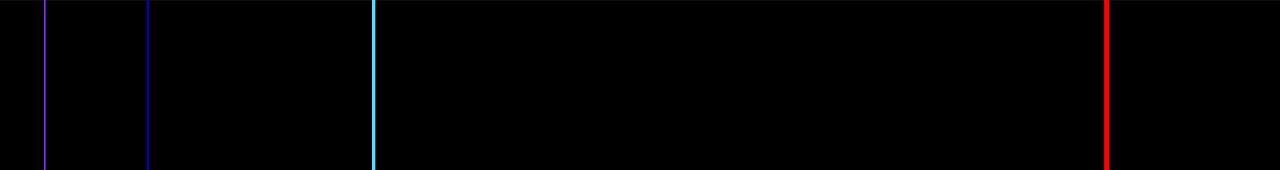
\includegraphics[width=0.70\linewidth]{images/book3/hydrogen-emission-spectrum.png}

{\small हाइड्रोजन का दृश्य उत्सर्जन वर्णक्रम: \qty{656}{nm}, \qty{486}{nm}, \qty{434}{nm} और \qty{410}{nm} पर बामर रेखाएँ, जिनमें से हर एक $n = 2$ तक की कोई छलाँग है।}
\end{omfigure}

\begin{omfigure}
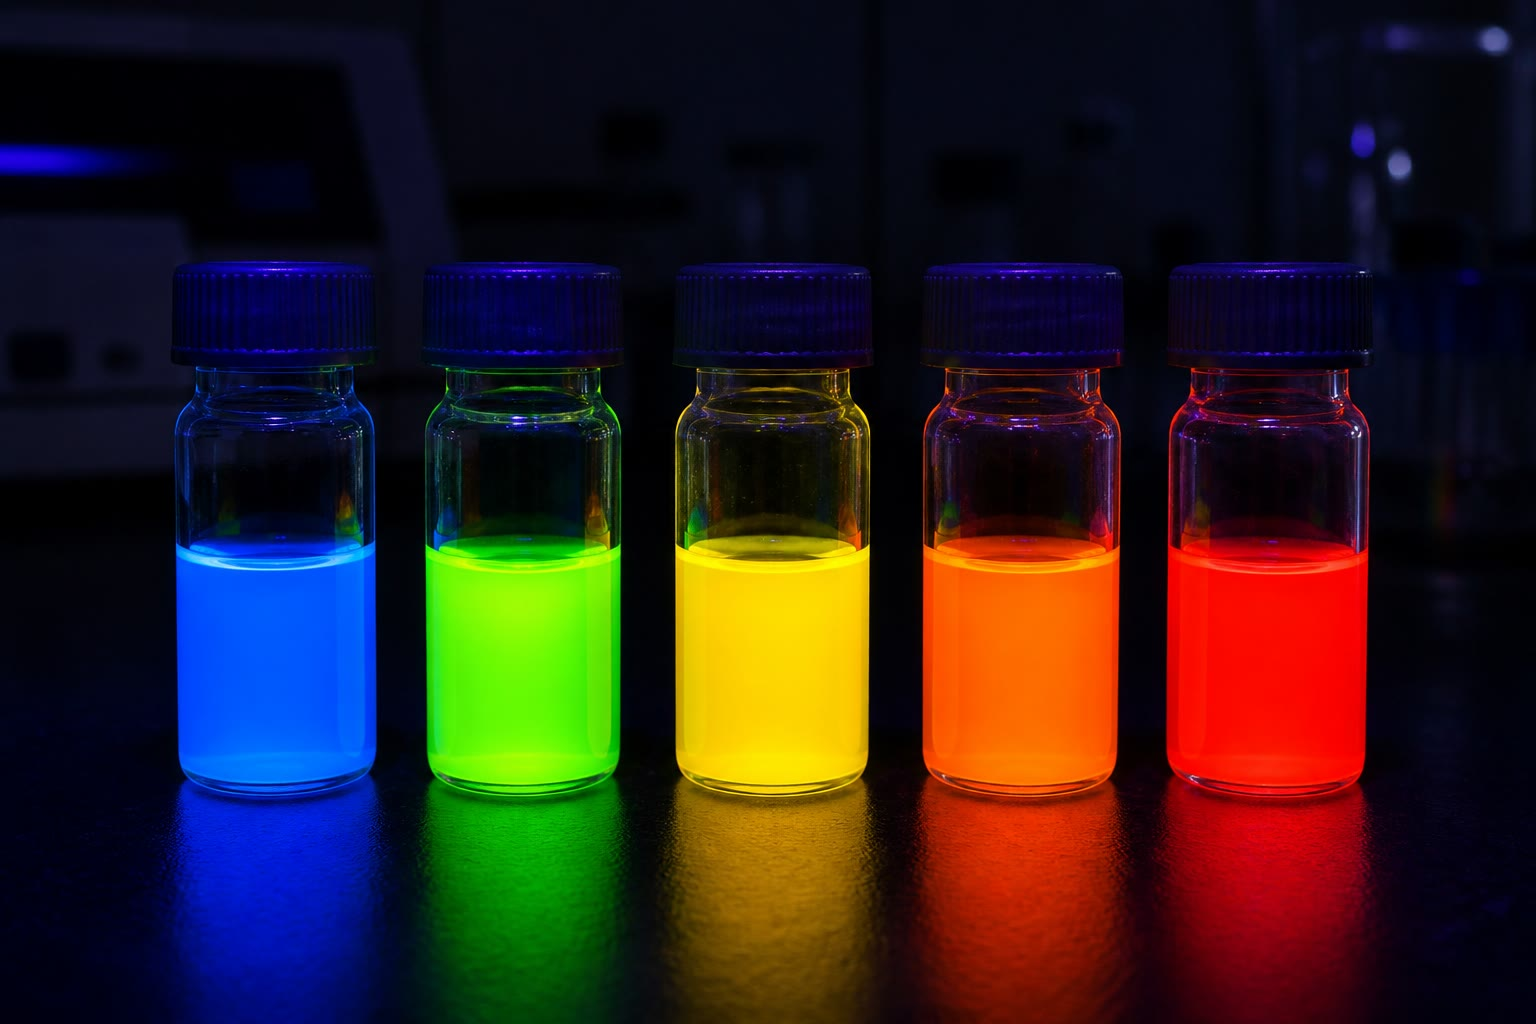
\includegraphics[width=0.60\linewidth]{images/book3/ai/b3-30-quantum-dots-vials.jpg}

{\small एक ही पदार्थ के \omterm{ex:b1:quantum-introduction:dot}{क्वांटम बिंदु} शीशियों में: नैनो-रवा जितना छोटा, बंदी-ऊर्जा उतनी बड़ी और प्रकाश उतना ही नीला --- यानी आकार से चुना गया रंग।}
\end{omfigure}

\section{समस्या: हाइड्रोजन का वर्णक्रम और एक क्वांटम बिंदु}

\begin{problem}[{सप्ताहांत समस्या --- प्रकाश और किसी वोल्टमापी से $h$ मापना,
तीन नियतांकों से हाइड्रोजन परमाणु खड़ा करना, और किसी रवे का रंग उसके आकार से
चुनना}]
\label{pb:b1:quantum-introduction:1}
नियतांक: $h = \qty{6.626e-34}{J.s}$, $\hbar = \qty{1.055e-34}{J.s}$, $c =
\qty{3.00e8}{m/s}$, $e = \qty{1.602e-19}{C}$, $m_e = \qty{9.11e-31}{kg}$,
$1/4\pi\varepsilon_0 = \qty{8.99e9}{SI}$, $hc = \qty{1240}{eV.nm}$।

\medskip
\noindent\textbf{भाग I --- \omterm{thm:b1:quantum-introduction:photon}{प्लांक नियतांक} मापना।}
पोटैशियम के किसी प्रकाश-कैथोड पर एकवर्णी प्रकाश डाला जाता है; और \omterm{prop:b1:quantum-introduction:photoelectric}{निरोधी
विभव} मापा जाता है: \qty{6.0e14}{Hz} पर \qty{0.30}{V}, \qty{7.0e14}{Hz} पर
\qty{0.69}{V}, \qty{8.0e14}{Hz} पर \qty{1.13}{V}, \qty{9.0e14}{Hz} पर
\qty{1.50}{V}, और \qty{1.1e15}{Hz} पर \qty{2.36}{V}।
\begin{enumerate}
  \item सेल का वर्णन कीजिए और समझाइए कि कोई उलटी वोल्टता धारा क्यों रोक
        सकती है, और $eV_s$ क्या मापता है।
  \item आइंस्टाइन का संबंध लिखिए और बताइए कि $V_s(\nu)$ की ढाल और
        अंतःखंड क्या देते हैं।
  \item आँकड़ों से (किसी रैखिक फ़िट से, या दोनों चरम बिंदुओं से)
        $h$ निकालिए; और स्वीकृत मान से तुलना कीजिए।
  \item पोटैशियम का कार्य-फलन \omterm{def:b1:charged-particles:eV}{इलेक्ट्रॉन-वोल्ट} में; देहली आवृत्ति और
        तरंगदैर्घ्य; और क्या कोई लाल लेज़र-सूचक इलेक्ट्रॉन निकाल सकता है?
  \item बत्ती की तीव्रता दुगुनी कर दी जाती है: $V_s$ का क्या होता है, और
        धारा का? यह किसी विशुद्ध तरंग-चित्र से असंगत क्यों है?
  \item चिरसम्मत आकलन: \qty{1}{\micro W/m^2} का कोई प्रकाश धातु पर पड़ता
        है; और कोई परमाणु लगभग \qty{1e-20}{m^2} का क्षेत्रफल देता है: तो
        किसी एक परमाणु पर \qty{2.2}{eV} जमा होने में कितना समय लगता? इसकी
        जगह देखा क्या जाता है?
\end{enumerate}

\medskip
\noindent\textbf{भाग II --- बोर का \omterm{prop:b1:quantum-introduction:hydrogen}{हाइड्रोजन परमाणु}।}
\begin{enumerate}[resume]
  \item किसी स्थिर प्रोटॉन के चारों ओर $r$ त्रिज्या की \omterm{prop:b1:central-forces:effective}{वृत्तीय कक्षा} पर
        कोई इलेक्ट्रॉन: चाल $v(r)$ और \omterm{thm:b1:work-and-energy:em}{यांत्रिक ऊर्जा} $E(r)$।
  \item बोर की शर्त $m_evr = n\hbar$: दिखाइए कि $r_n = n^2a_0$ है, और
        $a_0 = 4\pi\varepsilon_0\hbar^2/m_ee^2$ का मान दीजिए।
  \item $E_n = E_1/n^2$, जहाँ $E_1 = -m_ee^4/[2(4\pi\varepsilon_0)^2\hbar^2]$;
        \omterm{def:b1:charged-particles:eV}{इलेक्ट्रॉन-वोल्ट} में उसका मान।
  \item पहली कक्षा पर चाल और अनुपात $v_1/c$ (यानी सूक्ष्म-संरचना नियतांक
        $\alpha \approx 1/137$)।
  \item रेखाओं $2 \to 1$ (लाइमन $\alpha$), $3 \to 2$ और
        $4 \to 2$ (बामर H$\alpha$, H$\beta$) की तरंगदैर्घ्य: इनमें कौन दृश्य हैं?
  \item दिखाइए कि $1/\lambda = R_H(1/n^2 - 1/p^2)$ है और रिडबर्ग नियतांक
        $R_H$ निकालिए; तथा सबसे छोटी बामर तरंगदैर्घ्य।
  \item \omterm{prop:b1:quantum-introduction:box}{मूल अवस्था} से हाइड्रोजन की आयनन ऊर्जा; और उस फ़ोटॉन की तरंगदैर्घ्य
        जो उसे ठीक-ठीक आयनित कर दे।
  \item दे ब्रॉय: दिखाइए कि कक्षा $n$ की परिधि $n$ तरंगदैर्घ्य है --- यानी
        बोर की शर्त कोई अप्रगामी-तरंग शर्त ही है।
  \item यह प्रतिरूप जो दो बातें ग़लत बताता है, जो एक बात ठीक-ठीक बताता है,
        और पूरे सिद्धांत में कक्षा की जगह क्या ले लेता है।
\end{enumerate}

\medskip
\noindent\textbf{भाग III --- \omterm{ex:b1:quantum-introduction:dot}{क्वांटम बिंदु}।}
$R$ त्रिज्या का कोई कैडमियम सेलेनाइड नैनो-रवा किसी उत्तेजित इलेक्ट्रॉन को
(प्रभावी द्रव्यमान $m_e^\ast = 0.13\,m_e$) और उसके छोड़े हुए विवर को
($m_h^\ast = 0.45\,m_e$) बंद रखता है; और $R$ त्रिज्या के किसी गोले में हर
एक की बंदी-ऊर्जा $h^2/8m^\ast R^2$ है (स्वीकृत); थोक कैडमियम सेलेनाइड का अंतराल
$E_g = \qty{1.74}{eV}$ है।
\begin{enumerate}[resume]
  \item अप्रगामी-तरंग शर्त से किसी एक-विमीय डिब्बे में कण की ऊर्जाएँ
        $E_n = n^2h^2/8mL^2$ व्युत्पन्न कीजिए, और गोले वाले सूत्र से
        उसकी समानता पर टिप्पणी कीजिए।
  \item $R = \qty{2.0}{nm}$ के लिए इलेक्ट्रॉन की और विवर की बंदी-ऊर्जाएँ।
  \item $R = \qty{2.0}{nm}$, \qty{3.0}{nm} और \qty{4.0}{nm} के लिए छोड़े गए
        फ़ोटॉन की ऊर्जा तथा तरंगदैर्घ्य; और रंग।
  \item एक वाक्य में समझाइए कि छोटे बिंदु अधिक नीले क्यों होते हैं।
  \item \omterm{thm:b1:quantum-introduction:heisenberg}{अनिश्चितता सिद्धांत} से \omterm{def:b1:units-dimensions:oom}{परिमाण की कोटि} जाँचिए:
        इलेक्ट्रॉन के लिए $\Delta p \sim \hbar/R$, $R = \qty{2}{nm}$ पर, और
        उससे निकलती \omterm{thm:b1:work-and-energy:ke}{गतिज ऊर्जा}।
  \item कोई बिंदु \qty{577}{nm} पर \qty{1.0}{nW} छोड़ता है: प्रति सेकंड
        फ़ोटॉन।
\end{enumerate}

\medskip
\noindent\textbf{भाग IV --- क्वांटम गिनना।}
\begin{enumerate}[resume]
  \item \qty{633}{nm} पर \qty{1.0}{mW} के किसी लेज़र से प्रति सेकंड फ़ोटॉन।
  \item अँधेरे की अभ्यस्त आँख \qty{500}{nm} पर लगभग $100$ फ़ोटॉनों की कौंध
        पकड़ लेती है, जो \qty{0.1}{s} के भीतर आएँ: उससे संगत शक्ति।
  \item कोई एफ़एम एंटीना \qty{100}{MHz} पर \qty{1.0}{pW} पाता है: प्रति
        सेकंड फ़ोटॉन; क्या उन्हें एक-एक करके संसूचित करने की कोई आशा है?
  \item सार दीजिए: केवल $h$, $e$, $m_e$ से इस समस्या ने परमाणु-जगत की
        कौन-सी तीन राशियाँ निकालीं, और किन परिमाणों के साथ?
\end{enumerate}
\end{problem}
